% !BIB TS-program = biber

\RequirePackage[l2tabu,orthodox]{nag}

% TODO: decide if one-sided/two-sided
%\documentclass[headsepline,footsepline,footinclude=false,fontsize=11pt,paper=a4,listof=totoc,bibliography=totoc,BCOR=12mm,DIV=12]{scrbook} % two-sided
\documentclass[headsepline,footsepline,footinclude=false,oneside,fontsize=11pt,paper=a4,listof=totoc,bibliography=totoc]{scrbook} % one-sided

% TODO: change thesis information
\newcommand*{\getUniversity}{Technische Universität München}
\newcommand*{\getFaculty}{Informatics}
\newcommand*{\getDegree}{Informatics}
\newcommand*{\getSchool}{Computation, Information and Technology}
\newcommand*{\getTitle}{Image Classification for Nazi Symbols}
\newcommand*{\getTitleGer}{Bildklassifikation zur Erkennung nationalsozialistischer Symbole}
\newcommand*{\getAuthor}{Zhiwei Zhang}
\newcommand*{\getDoctype}{Master's Thesis}
\newcommand*{\getSupervisor}{Prof. Dr. Jürgen Pfeffer}
\newcommand*{\getAdvisor}{Daniel Matter}
\newcommand*{\getKeywords}{keyword;another keyword;one more}
\newcommand*{\getSubmissionDate}{15.07.2025}
\newcommand*{\getSubmissionLocation}{Munich}

% TODO: change citation style in settings
\PassOptionsToPackage{table,svgnames,dvipsnames}{xcolor}

\usepackage[a-2u]{pdfx} % generate PDF/A: archival compliant, self-contained pdf
\usepackage[utf8]{inputenc}
\usepackage[T1]{fontenc}
\usepackage[sc]{mathpazo}
\usepackage[ngerman,american]{babel}
\usepackage[autostyle]{csquotes}
\usepackage[%
  backend=biber,
  url=false,
  style=alphabetic,
  maxnames=4,
  minnames=3,
  maxbibnames=99,
  giveninits,
  uniquename=init]{biblatex} % TODO: adapt citation style
\usepackage{graphicx}
\usepackage{scrhack} % necessary for listings package
\usepackage{listings}
\usepackage{lstautogobble}
\usepackage{tikz}
\usepackage{pgf-pie}
\usepackage{pgfplots}
\usepackage{pgfplotstable}
\usepackage[final]{microtype}
\usepackage{caption}
\usepackage[printonlyused]{acronym}
\usepackage{ifthen}
\usepackage{times}
\usepackage{latexsym}
\usepackage{subcaption}
\usepackage{multirow}
\usepackage{amsmath}
\usepackage{wrapfig,lipsum,booktabs}
\usepackage{xcolor}
\usepackage[para,online,flushleft]{threeparttable}
\usepackage{url}

\newcommand*{\fullref}[1]{\hyperref[{#1}]{\autoref*{#1}: \nameref*{#1}}} % One single link

\makeatletter
\def\TPT@doparanotes{\par
   \prevdepth\z@ \TPT@hsize
   \TPTnoteSettings
   \parindent\z@ \pretolerance 8
   \linepenalty 200
   \renewcommand\item[1][]{\relax\ifhmode \begingroup
       \unskip
       \advance\hsize 10em % \hsize is scratch register, based on real hsize
       \penalty -45 \hskip\z@\@plus\hsize \penalty-19
       \hskip .15\hsize \penalty 9999 \hskip-.15\hsize
       \hskip .01\hsize\@plus-\hsize\@minus.01\hsize
       \hskip 6em\@plus .3em
              %%%%%
      \endgroup\fi
      \tnote{##1}\,\ignorespaces}%
   \let\TPToverlap\relax
   \def\endtablenotes{\par}%
}


\graphicspath{ {./figures/} }
\usetikzlibrary{arrows.meta, positioning, shapes.geometric, matrix}



\hypersetup{hidelinks} % removes colored boxes around references and links

% for fachschaft_print.pdf
\makeatletter
\if@twoside
	\typeout{TUM-Dev LaTeX-Thesis-Template: twoside}
\else
	\typeout{TUM-Dev LaTeX-Thesis-Template: oneside}
\fi
\makeatother

\addto\extrasamerican{
	\def\lstnumberautorefname{Line}
	\def\chapterautorefname{Chapter}
	\def\sectionautorefname{Section}
	\def\subsectionautorefname{Subsection}
	\def\subsubsectionautorefname{Subsubsection}
}

\addto\extrasngerman{
	\def\lstnumberautorefname{Zeile}
}

% Themes
\ifthenelse{\equal{\detokenize{dark}}{\jobname}}{%
  % Dark theme
  \newcommand{\bg}{black} % background
  \newcommand{\fg}{white} % foreground
  \usepackage[pagecolor=\bg]{pagecolor}
  \color{\fg}
}{%
  % Light theme
  \newcommand{\bg}{white} % background
  \newcommand{\fg}{black} % foreground
}

\bibliography{bibliography}

\setkomafont{disposition}{\normalfont\bfseries} % use serif font for headings
\linespread{1.05} % adjust line spread for mathpazo font

% Add table of contents to PDF bookmarks
\BeforeTOCHead[toc]{{\cleardoublepage\pdfbookmark[0]{\contentsname}{toc}}}

% Define TUM corporate design colors
% Taken from http://portal.mytum.de/corporatedesign/index_print/vorlagen/index_farben
\definecolor{TUMBlue}{HTML}{0065BD}
\definecolor{TUMSecondaryBlue}{HTML}{005293}
\definecolor{TUMSecondaryBlue2}{HTML}{003359}
\definecolor{TUMBlack}{HTML}{000000}
\definecolor{TUMWhite}{HTML}{FFFFFF}
\definecolor{TUMDarkGray}{HTML}{333333}
\definecolor{TUMGray}{HTML}{808080}
\definecolor{TUMLightGray}{HTML}{CCCCC6}
\definecolor{TUMAccentGray}{HTML}{DAD7CB}
\definecolor{TUMAccentOrange}{HTML}{E37222}
\definecolor{TUMAccentGreen}{HTML}{A2AD00}
\definecolor{TUMAccentLightBlue}{HTML}{98C6EA}
\definecolor{TUMAccentBlue}{HTML}{64A0C8}

% Settings for pgfplots
\pgfplotsset{compat=newest}
\pgfplotsset{
  % For available color names, see http://www.latextemplates.com/svgnames-colors
  cycle list={TUMBlue\\TUMAccentOrange\\TUMAccentGreen\\TUMSecondaryBlue2\\TUMDarkGray\\},
}

% Settings for lstlistings
\lstset{%
  basicstyle=\ttfamily,
  columns=fullflexible,
  autogobble,
  keywordstyle=\bfseries\color{TUMBlue},
  stringstyle=\color{TUMAccentGreen},
  captionpos=b
}

\lstdefinelanguage{json}{
    numbers=left,
    numberstyle=\tiny\color{gray},
    stepnumber=1,
    numbersep=8pt,
    showstringspaces=false,
    breaklines=true,
    frame=single,
    backgroundcolor=\color{gray!10},
    literate=
     *{0}{{{\color{blue}0}}}{1}
      {1}{{{\color{blue}1}}}{1}
      {2}{{{\color{blue}2}}}{1}
      {3}{{{\color{blue}3}}}{1}
      {4}{{{\color{blue}4}}}{1}
      {5}{{{\color{blue}5}}}{1}
      {6}{{{\color{blue}6}}}{1}
      {7}{{{\color{blue}7}}}{1}
      {8}{{{\color{blue}8}}}{1}
      {9}{{{\color{blue}9}}}{1}
      {:}{{{\color{red}:}}}{1}
      {,}{{{\color{red},}}}{1}
      {"}{{{\color{black}"}}}{1}
}

\begin{document}

% Set page numbering to avoid "destination with the same identifier has been already used" warning for cover page.
% (see https://en.wikibooks.org/wiki/LaTeX/Hyperlinks#Problems_with_Links_and_Pages).
\pagenumbering{alph}
\input{pages/cover}

\frontmatter{}

\input{pages/title}
\input{pages/disclaimer}
\addcontentsline{toc}{chapter}{Acknowledgments}
\thispagestyle{empty}

\vspace*{20mm}

\begin{center}
    {\usekomafont{sectioning}\usekomafont{section} Acknowledgments}
\end{center}

\vspace{10mm}

%TODO: Acknowledgments

First and foremost, I would like to express my deepest gratitude to my wife for her unwavering support, patience,
and encouragement throughout the entire course of this thesis. Her belief in me made all the difference during
challenging times.

I would like to sincerely thank Professor Jürgen Pfeffer for giving me the opportunity to pursue this research topic
and for fostering an academic environment that encourages intellectual curiosity and critical thinking.

I would also like to thank Dr. Angelina Voggenreiter for her kind assistance in helping me explore and identify
potential thesis topics within the chair.

Special thanks go to my colleagues and my manager at Allianz for their flexibility, understanding, and
encouragement, which greatly helped me balance my professional and academic commitments.

I am especially grateful to my friend Dr.\ Cristian Alfonso Gonzales Mora for his thoughtful and detailed feedback
during the review process, which helped me significantly improve the quality of this thesis.

Finally, I acknowledge my supervisor, Daniel Matter, for his valuable guidance, constructive feedback, and
continuous support during the development of this work. His insights have been instrumental in shaping both the
technical and ethical dimensions of the thesis.

\cleardoublepage{}

\chapter{\abstractname}

The detection and classification of Nazi-related symbols in digital images are critical tasks in combating the
spread of extremist content and supporting social science research on hate speech. This thesis investigates modern
image classification methods for identifying Nazi symbols, including both binary classification (detecting whether
any Nazi symbol is present) and multi-class classification (identifying the specific symbol type). A curated dataset
was compiled, consisting of 99,435 non-Nazi images and 2,338 Nazi-related images spanning 22 symbol categories. Due
to limited examples in some classes, several were regrouped into a consolidated \textit{Neo-Nazi} category to
improve model learnability.

Multiple deep learning architectures were evaluated, including ResNet50, EfficientNet, Vision Transformers (ViT),
OpenCLIP, and Moondream. Additionally, classical machine learning models were explored using OpenCLIP visual
embeddings as input features. Model performance was assessed using standard metrics such as accuracy, precision,
recall, F1-score, and AUC-ROC.

Experimental results demonstrate that for the binary classification task, OpenCLIP embeddings combined with
classical classifiers achieved competitive performance while requiring significantly fewer computational resources.
However, in the multi-class classification task, this combination underperformed substantially compared to ViT and
YOLOv11, with YOLOv11 achieving the best overall performance in identifying specific symbol classes.

To support practical application, the best-performing models were integrated into an \ac{API} service. A CI/CD pipeline
was implemented to automate packaging and publishing of the service as a Docker image, enabling easy deployment by
researchers or institutions. This work provides a lightweight and effective solution for detecting Nazi symbols in
large-scale image datasets and contributes to broader efforts in content moderation and digital extremism research.

\microtypesetup{protrusion=false}
\tableofcontents{}
\microtypesetup{protrusion=true}

\mainmatter{}

% !TeX root = ../main.tex
% Add the above to each chapter to make compiling the PDF easier in some editors.

\chapter{Introduction}\label{chapter:introduction}

\section{Background}

Social media platforms have emerged as primary channels for the dissemination of vast quantities of multimedia
content, including images, text, and video. These digital streams provide a rich source of data for research in the
social sciences, particularly in fields such as political extremism, regional conflict analysis, and hate speech
detection. To facilitate such research, scholars often rely on web crawlers to harvest large datasets from online
platforms. However, the raw data collected through these methods are typically unstructured and lack semantic
annotation, requiring significant preprocessing to extract meaningful insights.

For image data in particular, classification serves as a critical preprocessing step, transforming unstructured
content into labeled datasets that are suitable for both quantitative and qualitative analysis. Among the various
categories of harmful or sensitive visual content, Nazi-related imagery remains especially salient. Symbols such as
the swastika, once co-opted by the German National Socialist regime (1933–1945), continue to function as enduring
emblems of hate and extremism. Additional symbols—such as the \ac{SS} bolts, the Black Sun (linked to fascist occult
ideologies), and the Siegrune—have been appropriated by modern neo-Nazi and far-right movements. These symbols
persist across digital platforms, where they are employed to signal ideological affiliation, propagate extremist
views, or incite violence. Given that many countries restrict or criminalize the display of such imagery, there is a
pressing need for automated detection tools to support content moderation and policy enforcement.

\section{Problem Statement}

The automatic detection and classification of Nazi symbols in images is critical for researchers, journalists, civil
society organizations, and online platforms working to monitor and mitigate the spread of extremist content. While
commercial image classification services exist, they are often proprietary, lack transparency, and entail high usage
costs—particularly for applications requiring large-scale image analysis or custom symbol detection. This presents a
significant barrier not for governments per se, but for non-state actors and research groups who often operate under
tight computational and financial constraints.
Even when national institutions have greater resources, scalability and cost-efficiency remain key considerations.
High-throughput image classification tasks, such as analyzing large volumes of online content or social media images
in near real-time, can demand substantial compute time and infrastructure. In practice, this limits the feasibility
of using closed, black-box services that are either too slow, too expensive to scale, or unsuitable for
customization. Moreover, reliance on opaque systems may hinder accountability and reproducibility—both essential in
research and regulatory contexts.
To address these challenges, there is a need for an open, transparent, and efficient image classification system
tailored specifically for Nazi symbol detection. Such a system should support both binary classification: detecting
presence/absence of Nazi imagery, and multi-class classification: identifying specific symbols, while remaining
lightweight and adaptable enough to run on accessible hardware like single-GPU workstations. The same requirements
apply across adjacent domains, including online extremism tracking, digital forensics, and platform content
moderation—making the solution broadly relevant beyond its immediate scope.

\section{Objectives}

This research aims to design, implement, and evaluate an efficient and robust image classification framework for the
automatic detection and categorization of Nazi symbols in visual media. While the immediate focus is on Nazi
iconography, the broader goal is to develop a generalizable and extensible approach that can be adapted to other
categories of extremist or harmful visual symbols. This makes the framework more useful across different
contexts—including civil society monitoring, journalism, and platform moderation—where flexibility and scalability
are essential.

The specific objectives of this study are as follows:

\begin{itemize}
\item Construct a curated dataset of approximately 100,000 images, encompassing both Nazi-related and non-Nazi
imagery to support supervised training and evaluation.
\item Annotate and structure the dataset to support both binary (presence/absence) and multi-class (specific symbol)
classification tasks.
\item Investigate a diverse range of \ac{DL} and multimodal models—including \ac{CNN}s, \ac{ViT}, and OpenCLIP
embeddings—combined with classical \ac{ML} algorithms for downstream classification.
\item Evaluate model performance using standard classification metrics (e.g., accuracy, precision, recall, F1-score,
AUC), and analyze the comparative strengths and limitations of each approach.
\item Develop a lightweight, modular \ac{API} service to enable efficient model inference via HTTP requests, thereby
supporting real-world deployment and integration.
\end{itemize}

While this study is constrained in terms of data coverage and computational resources, it proposes a scalable
frameworkthat can be repurposed for other extremist symbol detection tasks by updating the dataset and retraining or
fine-tuning the models. This generalizable design makes it especially suitable for actors operating in fast-changing
threat landscapes or under limited infrastructure.

\section{Scope and Limitations}

The visual symbols associated with Nazi and neo-Nazi ideologies are numerous and varied, both historically and in
contemporary usage. Given this diversity, it is challenging to construct a comprehensive dataset that captures all
such symbols. Instead, this study focuses on a representative subset of the most visually distinctive and commonly
encountered symbols. Specifically, the following classes are included: \textit{Black Sun}, \textit{Flash and Circle},
\textit{Broken Sun Cross}, \textit{The Happy Merchant}, \textit{Hitler}, \textit{Nazi Salute},
\textit{Atomwaffen Division Emblem}, \textit{Blood \& Honor Emblem}, \textit{Celtic Cross}, \textit{Combat 18 Emblem},
\textit{Golden Dawn}, \textit{Hammerskins Emblem}, \textit{Identitarian Movement Emblem}, \textit{Kolovrat},
\textit{National Rebirth of Poland Emblem}, \textit{Popular Front Emblem}, \textit{Yellow Badge}, \textit{Siegrune},
\textit{\ac{SS} Skull}, \textit{Sturmabteilung Emblem}, \textit{Swastika}, and \textit{Wolfsangel}.

The classification system is designed to support two core tasks:

\begin{enumerate}
  \item \textbf{Binary Classification:} Determining whether a given image contains any Nazi-related symbol.
  \item \textbf{Multi-Class Classification:} Identifying which specific symbol (among 13 predefined categories) is
  present in a given image found to have Nazi-related symbology.
\end{enumerate}

In addition to dataset limitations, there were also hardware constraints. All experiments were conducted on a single
consumer-grade GPU (NVIDIA RTX 4060Ti) with 16 GB of video memory. This limited the ability to fine-tune large
models or run memory-intensive experiments—particularly with transformer-based architectures (e.g., ViT) or
multimodal embeddings (e.g., OpenCLIP). These models were used in this study, but only in lightweight or partially
frozen configurations to stay within the available hardware limits. It also restricted the feasibility
of training multiple models in parallel for ensembling. As a result, priority was given to computationally efficient
architectures and lightweight training procedures that could fit within the available memory and runtime budget.

Despite these constraints, this work seeks to demonstrate the feasibility of developing effective, accessible, and
ethically responsible tools for the detection of extremist visual content. It is intended to support researchers,
content moderators, and policymakers in their efforts to monitor and counteract the dissemination of hate imagery
online.

\section{Thesis Structure}

This thesis is organized as follows:

\begin{itemize}
  \item \textbf{\fullref{chapter:literature-review}} – Surveys existing research on Nazi symbol detection and
  classification, emphasizing methodological trends, key findings, and identifying research gaps addressed in this work.

  \item \textbf{\fullref{chapter:methodology}} – Describes the data collection
  process, dataset composition, preprocessing techniques, and the used classification algorithms. It also
  outlines the model training process, evaluation metrics, and justifies the chosen methodologies.

  \item \textbf{\fullref{chapter:ethical-considerations}} – Discusses the ethical implications of working with sensitive
  content, including concerns around data privacy, potential misuse, and broader responsibilities associated with
  automated hate symbol detection.

  \item \textbf{\fullref{chapter:results}} – Presents the outcomes of the experiments, including both
  quantitative and qualitative analyses of model performance for binary and multi-class classification tasks.

  \item \textbf{\fullref{chapter:discussion-and-analysis}} – Interprets the results in relation to the
  research objectives, compares findings to prior work, and discusses system limitations and potential improvements.

  \item \textbf{\fullref{chapter:model-deployment-and-api-service}} – Describes the deployment strategy
  for the best-performing models, including the architecture of the \ac{API} service, the \ac{CI/CD} pipeline, and
  details of the available endpoints.

  \item \textbf{\fullref{chapter:conclusion-and-future-work}} – Summarizes the thesis contributions, reflects on key
  insights gained, and outlines directions for future research in the field of Nazi symbol classification.
\end{itemize}

\input{chapters/02_literature_review}
%! Author = zhiweizhang
%! Date = 10.06.25

\chapter{Ethical Considerations}\label{chapter:ethical-considerations}

The development of \ac{ML} systems for the classification of Nazi symbols entails a range of ethical
challenges due to the sensitive, harmful, and potentially illegal nature of the target content. These concerns
reflect broader societal expectations for responsible AI, as articulated in international frameworks such as \ac{UNESCO}’s
\textit{Recommendation on the Ethics of Artificial Intelligence}~\parencite{unesco2021}. This chapter
outlines the core ethical principles guiding the research, grounded in widely recognized frameworks such as the \ac{IEEE}
\textit{Ethically Aligned Design} guidelines~\parencite{ieee2021ethics}, the EU AI Act~\parencite{euai2023}, and the
\ac{DFG}’s \textit{Guidelines for Safeguarding Good Research Practice}~\parencite{dfg2022}. These considerations are
essential for ensuring that the study is conducted responsibly, complies with legal norms, and anticipates the
social implications of deploying such a system.

\begin{itemize}
    \item \textbf{Foundational Ethical Frameworks:} This research is informed by established ethical guidelines such
    as the IEEE Ethically Aligned Design~\parencite{ieee2021ethics} and the Belmont Report~\parencite{belmont1979},
    the latter—originally developed for biomedical research—offers enduring principles like
    respect for persons and beneficence that extend to socially impactful AI systems. These principles guide our
    handling of sensitive data and system design choices.

    \item \textbf{Handling of Sensitive Content:} Nazi symbols are strongly associated with hate, violence, and
    genocide. Datasets containing such imagery must be handled with care to avoid trivializing or normalizing hateful
    ideologies. Access to these datasets is strictly limited, and appropriate content warnings and disclaimers are used.
    Data management follows established protocols for working with sensitive or controversial materials, in accordance
    with research integrity standards outlined by the \ac{DFG}~\parencite{dfg2022}.

    \item \textbf{Purpose and Intent:} The goal of this research is to assist in identifying and moderating harmful
    content, not to promote or propagate extremist ideologies. Transparency in the project's objectives helps
    prevent misuse, aligning with principles of socially beneficial AI outlined by the \ac{IEEE} and
    \ac{UNESCO}~\parencite{ieee2021ethics,unesco2021}.

    \item \textbf{Legal Compliance:} In countries such as Germany and Austria, strict laws (e.g., Section 86a of the
    German Criminal Code) prohibit the display and distribution of Nazi symbols. This study complies with all
    applicable regulations, ensuring that content is accessed solely for legitimate research purposes and not
    redistributed~\parencite{bundesregierung2023}.

    \item \textbf{Data Sourcing and Annotation:} All datasets were collected from publicly available
    repositories—primarily Kaggle and Roboflow—which permit academic and non-commercial use under their respective
    licenses\footnote{Kaggle Terms of Service: \url{https://www.kaggle.com/terms}; Roboflow Terms:
    \url{https://roboflow.com/terms}}. No restricted or proprietary content was used. All annotations were conducted
    manually by the researcher. Content warnings were observed throughout the process to mitigate potential
    psychological distress, as also described in ~\autofullref{sec:data-construction} from ~\autofullref{chapter:methodology}.

    \item \textbf{Bias and Misclassification Risks:} Classification systems may mistakenly flag benign content or
    overlook altered forms of hate symbols. Such errors could lead to unjust moderation or missed threats. To
    address this, the study prioritized balanced training data, fairness-aware evaluation, and extensive model
    validation in line with AI fairness principles~\parencite{mehrabi2021survey}.

    \item \textbf{Dual-Use Concerns:} While developed for moderation purposes, such a classification system could be
    repurposed for malicious use, such as evading content filters or enabling authoritarian surveillance.
    Recognizing this dual-use risk~\parencite{brundage2018malicious}, the research limits model distribution and
    recommends transparency, access control, and red-teaming before deployment.

    \item \textbf{Privacy and Consent:} If any images included identifiable individuals, anonymization procedures
    were applied in accordance with \ac{GDPR} principles and ethical AI guidelines~\parencite{gdpr2016}. No \ac{PII}
    was intentionally collected or retained.

    \item \textbf{Transparency and Accountability:} All stages of the research—including data provenance,
    preprocessing, model selection, and limitations—are documented and disclosed. This transparency aligns with
    reproducible research norms and promotes accountability in the deployment of AI systems on sensitive
    content~\parencite{Mitchell_2019}.
\end{itemize}

\noindent
In sum, these ethical frameworks are not peripheral to the study but foundational to its design and execution. They
inform not only how data is sourced, labeled, and secured, but also how models are evaluated, interpreted, and
constrained in their use. With these considerations in place, the following chapter details the methodological
pipeline through which the classification system is developed and validated.

%! Author = zhiweizhang
%! Date = 10.06.25

\chapter{Methodology}\label{chapter:methodology}

In this section, we will discuss our training data first, then we
discuss about data preprocessing steps, at the end we talk about the
algorithms we used.

\section{Data Collection}
\label{sec:data-collection}

To develop a robust image classifier capable of distinguishing Nazi symbols from other visual elements, a
comprehensive dataset containing both positive and negative image classes was constructed. The datasets were sourced
from two major platforms:

\begin{itemize}
  \item \textbf{Roboflow}: Provided labeled datasets containing Nazi symbols such as swastikas, SS bolts, and the
  Black Sun. These datasets constituted the positive class and were selected based on symbol relevance, label
  accuracy, and visual diversity.

  \item \textbf{Kaggle}: Offered general-purpose datasets comprising everyday objects, street scenes, and
  non-extremist logos. These images formed the negative class, helping the model learn to discriminate between Nazi
  iconography and unrelated content, thereby minimizing false positives.
\end{itemize}

The collected datasets varied in resolution, label format, class granularity, and symbolic diversity. A summary
table including dataset names, descriptions, and sources is provided in Table~\autoref{tab:dataset_summary}.

All datasets were obtained under open-use or research-friendly licenses, in compliance with the terms specified by
their respective platforms and contributors. To ensure data integrity and ethical compliance, the following steps
were taken:

\begin{itemize}
  \item Manual inspection was performed on each dataset to verify label accuracy and image quality.
  \item Nazi symbol datasets were annotated and filtered into predefined classes based on visual traits and
  historical context, guided by taxonomies from the Anti-Defamation League (ADL) and academic research on hate iconography.
  \item Duplicate or near-duplicate images across datasets were removed to prevent data leakage.
\end{itemize}

The aggregated dataset was randomly partitioned into three subsets: 70\% for training, 15\% for validation, and 15\%
for testing. Care was taken to avoid overlap of symbol instances across these partitions.

\begin{table}[htbp]
\centering
\small
%\renewcommand{\arraystretch}{2}
\resizebox{\textwidth}{!}{
\begin{tabular}{clcl}
\toprule
\textbf{Platform} & \textbf{Dataset Name / Description} & \textbf{Purpose} & \textbf{Notes} \\
\midrule
Roboflow & detect Dataset~\parencite{detect-lhuia_dataset} & Positive Class & Swastika and related Nazi symbols \\

Roboflow & swastika Dataset (imgann)~\parencite{swastika-o7bde_dataset} & Positive Class & Swastika symbol detection \\

Roboflow & swastika Dataset (Darja Nechaeva)~\parencite{swastika-uw8xt_dataset} & Positive Class & Historical swastika variations \\

Roboflow & swastika\_detect Dataset~\parencite{swastika_detect_dataset} & Positive Class & Swastika detection for moderation \\

Roboflow & symbols Dataset~\parencite{symbols-w93jw_dataset} & Positive Class & Includes general and hate symbols \\

Roboflow & violent object Dataset~\parencite{violent-object_dataset} & Positive Class & Hate symbols and violent imagery \\

Roboflow & Swastiki\_Net Dataset~\parencite{swastiki_net_dataset} & Positive Class & Swastika symbol classification \\

Roboflow & Content Moderation Dataset~\parencite{content-moderation-fwj5b_dataset} & Positive Class & Multiple harmful or extremist symbols \\

Roboflow & Swastika\_Detection Dataset~\parencite{swastika_detection_dataset} & Positive Class & Swastikas in different contexts \\

Kaggle & 100 Sports Image Classification~\parencite{100_sport_image_classification_dataset} & Negative Class & Neutral sports images \\

Kaggle & Car vs Bike Classification Dataset~\parencite{car_bike_classification_dataset} & Negative Class & Background class diversity \\

Kaggle & People Clothing Segmentation~\parencite{people_clothing_segmentation_dataset} & Negative Class & Background objects, neutral content \\

Kaggle & Fruits and Vegetables Dataset~\parencite{fruit_and_vegetable_image_recognition_dataset} & Negative Class & For reducing false positives \\

Kaggle & Animal Image Dataset~\parencite{animal_image_dataset} & Negative Class & Animal images for neutral comparison \\

Kaggle & Kids and Adults Detection~\parencite{kids_and_adults_detection_dataset} & Negative Class & Human figures, non-extremist \\

Kaggle & SCOOBY DOO Classification~\parencite{scooby_doo_classification_dataset} & Negative Class & Cartoon data for variance \\

Kaggle & Low Light Animals~\parencite{subrata_sarkar_2025} & Negative Class & Low-light conditions for robustness \\

Kaggle & AI vs Human-Generated Images~\parencite{ai_vs_human_generated_images_dataset} & Negative Class & Diverse image source simulation \\
\bottomrule
\end{tabular}
}
\caption{Summary of datasets used in this thesis for training, validation, and testing.}
\label{tab:dataset_summary}
\end{table}

\subsection{Nazi Symbol Taxonomy and Distribution}

The final dataset includes \textbf{22 distinct Nazi-related symbols}, ranging from widely recognized emblems (e.g.,
swastika, SS bolts) to lesser-known variants (e.g., Wolfsangel, Kolovrat). These were selected based on their
documented use in historical Nazi insignia, far-right propaganda, and contemporary neo-Nazi subcultures. A visual
overview of representative images is shown in Figure~\ref{figure:nazi-symbol-examples}, while
Section~\autoref{section:symbol-description} provides full symbol descriptions.

\begin{figure}[ht]
  \centering
  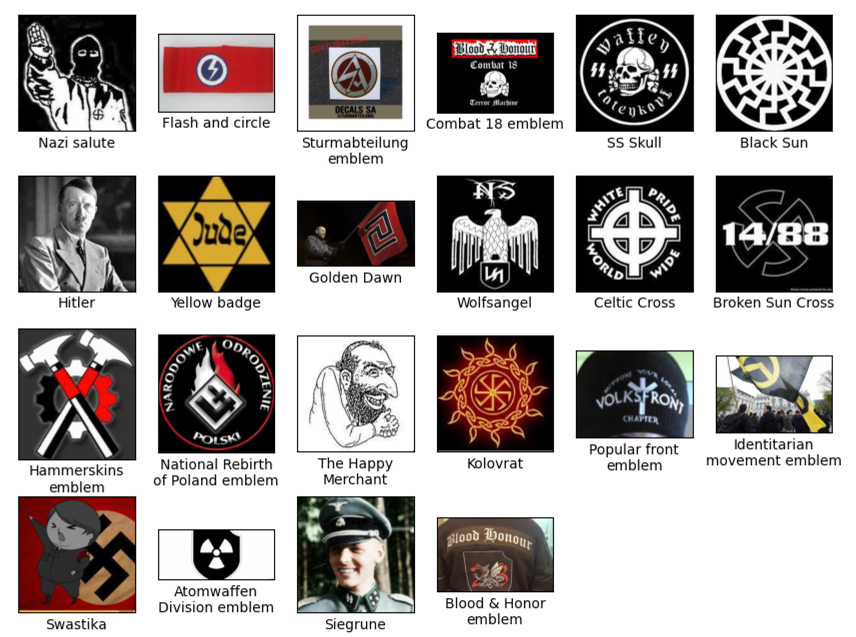
\includegraphics[scale=0.55]{nazi-symbol-examples}
  \caption{Example images from 22 Nazi symbol classes.}
  \label{figure:nazi-symbol-examples}
\end{figure}

\section{Nazi Symbol Description}
  \label{section:symbol-description}

The Nazi symbols are mainly from Roboflow with labels. The symbols are defined as follows:

\begin{itemize}
  \item \textbf{Sonnenrad}: The sonnenrad, or sunwheel, is an ancient symbol
  from Norse and Celtic cultures that was appropriated by the Nazis to
  promote an idealized "Aryan" heritage. Its many variations include forms
  of the swastika and Celtic Cross, and it was used by the Nazi Party,
  SA, and SS. Today, it is commonly used by neo-Nazis and white
  supremacists, especially a version with two concentric circles and
  crooked rays, sometimes featuring a swastika in the center.
  \item \textbf{Flash and circle}: The Flash and Circle is a symbol featuring
  a lightning bolt within a circle, originally used by the British Union
  of Fascists in the 1930s. It was meant to represent action within unity
  and has since been adopted by neo-fascist and white supremacist groups.
  Though less common today, it remains a recognizable hate symbol associated
  with fascist ideology.
  \item \textbf{Broken Sun Cross}: Symbols featuring an equilateral cross enclosed
  in a circle have appeared in various cultures since the Bronze Age. Since
  the 1930s, a version with ‘broken’ arms resembling a swastika gained far-right
  associations. It was used by the German Faith Movement and later as insignia
  for two Waffen SS divisions.
  \item \textbf{The Happy Merchant}: The Happy Merchant is an antisemitic meme
  depicting a Jewish man with exaggerated, stereotypical features, often used
  by white supremacists to promote hate. It originated from racist artwork
  by cartoonist Nick Bougas, who used the pseudonym “A. Wyatt Mann.” His
  offensive cartoons, widely circulated in the 1980s and 1990s, were often
  published by white supremacist Tom Metzger.
  \item \textbf{Hitler}: The images of Adolf Hilter.
  \item \textbf{Nazi salute}: The Nazi salute, also known as the Hitler salute
  or Sieg Heil salute, was a gesture used
  in Nazi Germany to show loyalty to Adolf Hitler and the Nazi Party, typically
  accompanied by phrases like "Heil Hitler" or "Sieg Heil". Inspired by the
  Italian Fascist salute, it became an official Nazi greeting in 1926 and
  was mandatory for civilians but optional for military personnel until
  1944. Today, the salute is banned in several countries—including Germany,
  Austria, and Slovakia—and is considered hate speech or a criminal act in
  many others if used to promote Nazi ideology.
%  \item \textbf{Neo-Nazi emblems}: Neo-Nazi emblems are symbols used by modern
%    white supremacist and neo-Nazi groups to express their extremist beliefs
%    and allegiance to Nazi ideology. These emblems often include modified or
%    obscure versions of historical Nazi symbols, such as the swastika, sonnenrad,
%    or runes, to avoid legal restrictions or public scrutiny. While some are
%    direct revivals, others are new creations that serve the same purpose of
%    spreading hate and promoting white nationalist ideas. In this study, it includes
%    symbols from various far-right extremist groups, such as Atomwaffen Division emblem,
%    Blood \& Honor emblem, Celtic Cross, Combat 18 emblem, Golden Dawn, Hammerskins emblem,
%    Identitarian movement emblem, Kolovrat, National Rebirth of Poland emblem,
%    Popular front emblem. Since only a limited number of images were available for
%    each group, they were consolidated under a single "Neo-Nazi" class for classification purposes.
  \item \textbf{Yellow badge}: The Yellow badge was a cloth patch, usually in
  the shape of a Star of David, that Jews were forced to wear by the Nazis
  to identify and segregate them. It symbolized persecution and was used to
  mark Jews publicly, contributing to their dehumanization and eventual
  deportation. Today, it stands as a powerful symbol of the Holocaust and
  the oppression of Jewish people.
  \item \textbf{Siegrune}: The Siegrune, or "S rune", is a lightning-bolt-shaped
  symbol used by the Nazi SS to represent victory ("Sieg" in German). It was
  adapted from ancient runic alphabets and became one of the most recognizable
  symbols of the SS, often displayed as a double rune on uniforms and insignia.
  Today, it is widely recognized as a hate symbol and is banned or restricted
  in several countries due to its association with Nazi ideology.
  \item \textbf{SS Skull}: The SS skull, also known as the "Totenkopf" ("death's head"),
  was a symbol used by the Nazi SS to represent loyalty unto death and intimidation.
  It was prominently featured on SS uniforms, especially those of the elite units
  and concentration camp guards. Today, it is considered a hate symbol due to
  its strong association with the crimes and ideology of the SS and the Nazi regime.
  \item \textbf{Sturmabteilung emblem}: The Sturmabteilung (SA) emblem was the
  symbol of the Nazi Party's paramilitary wing, known for its violent tactics
  and support for Adolf Hitler's rise to power. The emblem typically featured
  a stylized version of the SA initials, often accompanied by a swastika.
  It represented the SA's role in enforcing Nazi ideology and intimidation,
  and the emblem is now recognized as a symbol of hate and fascism.
  \item \textbf{Swastika}: The Swastika is an ancient symbol, originally used in
  various cultures to represent good luck, prosperity, and well-being. However,
  it was appropriated by the Nazi Party in the 1920s, becoming a powerful
  symbol of their ideology and representing white supremacy, hate, and
  anti-Semitism. Today, it is widely recognized as a symbol of Nazi oppression
  and is illegal in many countries due to its association with hate and violence.
  \item \textbf{Wolfsangel}: The Wolfsangel is a symbol originally used in medieval
  Europe, representing a wolf trap, and later adopted by Nazi and neo-Nazi
  groups. It was used by Nazi units during World War II, including the Waffen-SS,
  and has become associated with white supremacy and fascist ideologies. Today,
  the Wolfsangel is a recognized hate symbol, often used by extremist groups
  to promote Nazi beliefs.
  \item \textbf{Atomwaffen Division emblem}:The Atomwaffen Division emblem is a symbol
  used by a violent neo-Nazi terrorist group known for promoting accelerationism and
  engaging in acts of domestic terrorism. The emblem typically features a stylized
  radiation warning symbol, representing the group's fascination with chaos,
  destruction, and nuclear war. It is widely recognized as a hate symbol and is
  associated with extremist violence, white supremacy, and far-right terrorism.
  \item \textbf{Blood \& Honor emblem}: The Blood \& Honour emblem represents an international
  neo-Nazi network that promotes white supremacist music and ideology. The name comes
  from the Hitler Youth motto "Blut und Ehre" (Blood and Honor), and the emblem often
  includes those words along with fascist symbols like runes or laurel wreaths. It
  is widely recognized as a hate symbol linked to racist propaganda, violence,
  and far-right extremism.
  \item \textbf{Celtic Cross}: The Celtic Cross is an ancient symbol with religious
  and cultural origins in Celtic Christianity, featuring a cross with a circle
  around the intersection. While it remains a legitimate cultural and religious
  symbol, white supremacists have adopted a simplified version as a symbol of white
  identity and nationalism. This version is now widely recognized as a hate symbol
  in extremist contexts.
  \item \textbf{Combat 18 emblem}: Combat 18 is a violent neo-Nazi organization, with the
  number "18" representing the initials A and H (Adolf Hitler). Its emblem typically
  includes the number or stylized letters alongside other far-right imagery. The group
  is known for promoting white supremacy and terrorism, and its emblem is a symbol of
  hate and violence.
  \item \textbf{Golden Dawn}: Golden Dawn is a far-right political party from Greece known for its neo-Nazi ideology
  and involvement in violent, xenophobic acts. Its emblem resembles a Greek meander pattern, often compared to a
  swastika due to its stylized, angular design. Though once politically active, the group has been widely condemned
  and legally prosecuted for its extremist activities.
  \item \textbf{Hammerskins emblem}: The Hammerskins emblem features two crossed hammers, symbolizing the group's
  slogan "Hammerskins Nation" and white power. This violent white supremacist group is rooted in the skinhead
  movement and is heavily involved in hate music and racist activism. The emblem is a well-known hate symbol tied to
  global neo-Nazi networks.
  \item \textbf{Identitarian movement emblem}: The Identitarian Movement emblem typically features a yellow circle
  with a black Greek lambda symbol, inspired by the Spartan shield. This far-right European movement promotes
  anti-immigration and ethnonationalist ideologies under the guise of cultural preservation. Although presented with
  modern, clean branding, the emblem is associated with white nationalist beliefs.
  \item \textbf{Kolovrat}: The Kolovrat is an ancient Slavic symbol representing the sun and cosmic cycles, used
  historically in pagan contexts. In recent years, it has been appropriated by Slavic neo-Nazis and white
  supremacists as a symbol of ethnic purity and nationalist pride. While some use it in a cultural or historical
  sense, its association with extremist ideology marks it as a hate symbol in certain contexts.
  \item \textbf{National Rebirth of Poland emblem}: The National Rebirth of Poland (NOP) emblem represents a
  far-right nationalist party in Poland known for its anti-Semitic and xenophobic views. The emblem often
  incorporates stylized nationalist imagery, including swords or eagles, designed to evoke Polish strength and
  purity. It is associated with extremist rhetoric and far-right political activism in Poland.
  \item \textbf{Popular front emblem}: The Popular Front emblem is used by a range of nationalist or fascist groups,
  often combining traditional nationalist symbols like eagles or stars with militaristic imagery. Though the term "
  Popular Front" historically referred to leftist coalitions, in extremist contexts, it can represent
  ultra-nationalist, anti-democratic movements. The emblem typically signals far-right or authoritarian ideologies.
%  \item \textbf{Doppelsiegrune}: The Doppelsiegrune, or "double Siegrune," features two lightning-bolt-like runes
%  and was the official insignia of the Nazi SS. It symbolized power, obedience, and loyalty to Adolf Hitler and
%  became one of the most infamous emblems of the Nazi regime. Today, it is banned or heavily restricted in many
%  countries and is recognized worldwide as a symbol of hate and terror.
\end{itemize}

\subsection{Dataset Structuring for Tasks}

To accommodate the differing objectives of the binary and multi-class classification tasks, the dataset was
structured as follows:

\begin{itemize}
    \item \textbf{Binary Classification (Symbol Detection):}
    All images containing any of the 22 Nazi-related symbol classes were merged into a single positive class labeled
    \item \textit{Nazi}. Images without Nazi-related content were labeled as \textit{non-Nazi}.
    The resulting dataset consisted of approximately \textbf{2,300 Nazi images} and \textbf{99,000 non-Nazi images},
    reflecting a 1:42 class ratio. This structuring supports a general detection task, identifying whether any Nazi
    symbol is present in an image.

    \item \textbf{Multi-Class Classification (Symbol Identification):}
    This task focused exclusively on the 22 Nazi symbol categories. Only images labeled with a Nazi symbol were
    included, preserving their individual class labels.
    The dataset for this task included a total of approximately \textbf{2,300 images}, with class sizes ranging from
    tens to hundreds of examples per symbol. Due to this variability, the dataset exhibited significant class
    imbalance, which posed challenges for model generalization across all symbol categories.
\end{itemize}

This structuring strategy ensured that the dataset aligned with the goals of each classification task: broad
detection capability in the binary case and fine-grained categorization in the multi-class case.


Due to the limited number of images in several classes, a new category labeled \textit{Neo-Nazi} was created to
group together symbol classes with very few examples. This regrouping allows the classifier to generalize better and
prevents overfitting on sparsely represented classes. Table~\autoref{tab:symbol-distribution} presents the distribution
of images in both the main Nazi-related symbol classes and the individual symbol types grouped under the
\textit{Neo-Nazi} label. The regrouping also improves class balance in the multi-class classification task, while
retaining interpretability for downstream applications.

%! Author = zhiweizhang
%! Date = 10.06.25

% Preamble
\begin{table}[ht]
  \begin{subtable}[c]{0.5\textwidth}
    \centering
    \begin{tabular}{|l|c|}
      \hline
      \textbf{Class} & \textbf{Images} \\
      \hline\hline
      Sonnenrad & 152 \\\hline
      Flash and circle & 13 \\\hline
      Broken Sun Cross & 21 \\\hline
      The Happy Merchant & 39 \\\hline
      Hitler & 228 \\\hline
      Nazi salute & 6 \\\hline
      Neo-Nazi & 188 \\\hline
      Yellow badge & 4 \\\hline
      Siegrune & 311 \\\hline
      SS Skull & 257 \\\hline
      Sturmabteilung emblem & 11 \\\hline
      Swastika & 1070 \\\hline
      Wolfsangel & 38 \\\hline
    \end{tabular}
    \subcaption{Regrouped symbol distribution}
  \end{subtable}
\hfill
  \begin{subtable}[c]{0.5\textwidth}
    \centering
    \begin{tabular}{|l|c|}
      \hline
      \textbf{Class} & \textbf{Images} \\
      \hline\hline
      Atomwaffen Division & 8 \\\hline
      Blood \& Honor emblem & 25 \\\hline
      Celtic Cross & 51 \\\hline
      Combat 18 emblem & 6 \\\hline
      Golden Dawn & 19 \\\hline
      Hammerskins emblem & 12 \\\hline
      Identitarian movement & 11 \\\hline
      Kolovrat & 38 \\\hline
      National Rebirth of Poland & 10 \\\hline
      Popular Front emblem & 8 \\\hline
    \end{tabular}
    \subcaption{Neo-Nazi Symbol distribution}
  \end{subtable}

  \caption{Symbol distribution}
  \label{tab:symbol-distribution}
\end{table}

\subsection{Sample Images}

Figure~\autoref{fig:dataset-samples} presents representative examples from both classes, illustrating the visual
diversity and annotation consistency.

\begin{figure*}[ht]
  \centering
  \begin{subfigure}[t]{0.48\textwidth}
    \centering
    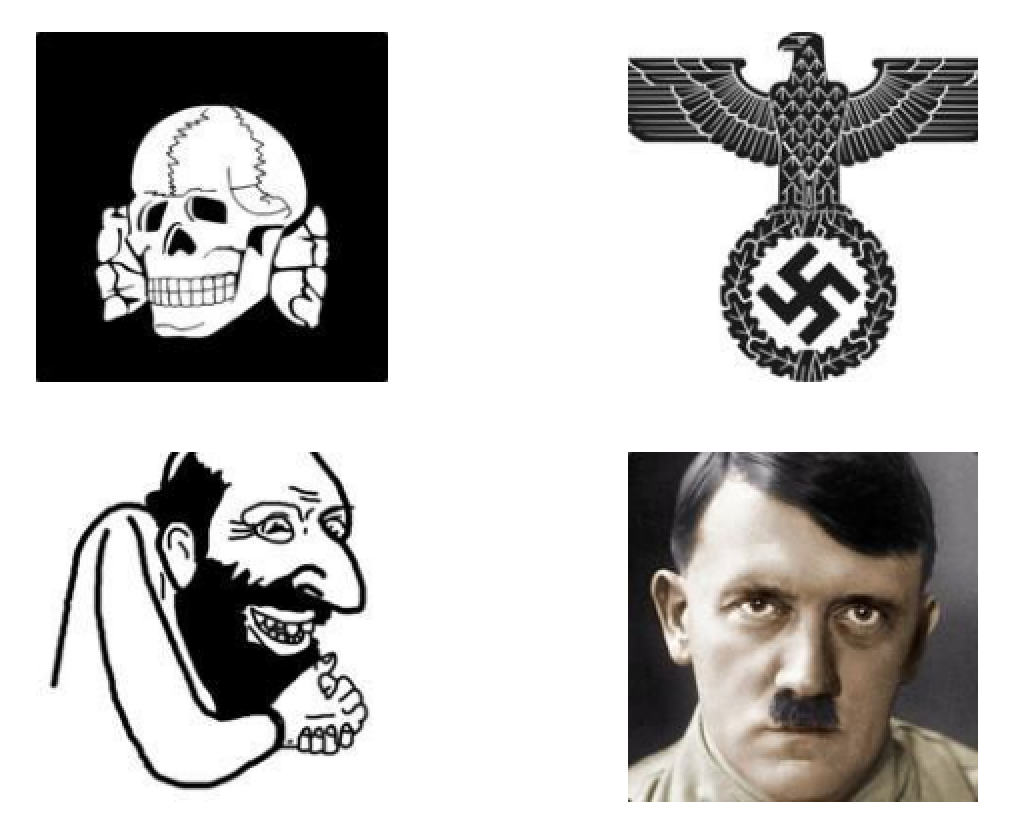
\includegraphics[scale=0.37]{nazi-examples}
    \caption{Sample images containing Nazi symbols}
  \end{subfigure}%
  \hfill
  \begin{subfigure}[t]{0.48\textwidth}
    \centering
    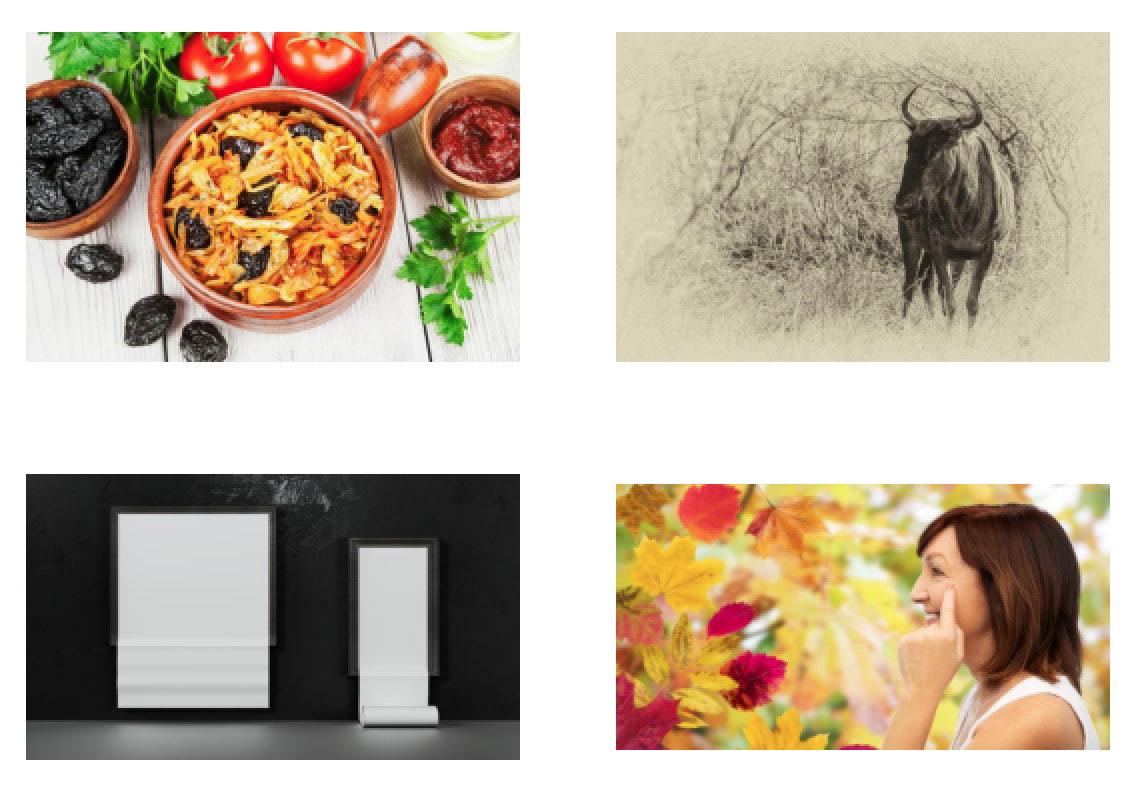
\includegraphics[scale=0.39]{non-nazi-examples}
    \caption{Sample images not containing Nazi symbols}
  \end{subfigure}
  \caption{Examples from the positive and negative classes}
  \label{fig:dataset-samples}
\end{figure*}

\noindent
All data collection procedures were conducted in accordance with academic ethical standards. No personal or
sensitive identifiable content was included, and all datasets were used strictly for research purposes aimed at
countering extremism.

\section{Algorithms}
To evaluate the effectiveness of different machine learning approaches in Nazi symbol detection and classification,
we experimented with a diverse set of models. These include both modern deep learning architectures and traditional
machine learning algorithms, allowing us to compare performance across various paradigms and computational complexities.

\subsection{YOLO (You Only Look Once)}
YOLO is a real-time object detection framework that treats detection as a single regression problem, directly
predicting bounding boxes and class probabilities from full images. YOLO processes the entire image in one forward
pass, offering a trade-off between speed and accuracy that is well-suited for applications requiring real-time
inference. While primarily intended for detection tasks, YOLO can be adapted for classification by interpreting the
most confident detection as the image label. In this study, we adopt YOLOv11 for its enhanced speed and robustness,
leveraging its latest improvements in backbone design and label assignment.

\subsection{ResNet (Residual Network)}
ResNet is a convolutional neural network that employs residual learning to ease the training of very deep networks
by introducing identity shortcut connections. This design mitigates the vanishing gradient problem, enabling
efficient training of architectures with hundreds of layers. ResNet has demonstrated strong performance in image
classification benchmarks. We utilize ResNet-50, a 50-layer deep variant, for its proven balance between model
complexity and classification accuracy.

\subsection{EfficientNet}
EfficientNet is a family of CNN architectures that systematically scales depth, width, and resolution using a
compound coefficient, resulting in a series of models that achieve state-of-the-art accuracy with significantly
fewer parameters. EfficientNet is highly efficient in resource usage, making it suitable for large-scale image
classification on limited hardware. In our experiments, it serves as a lightweight alternative to deeper networks
without substantial sacrifice in accuracy.

\subsection{Vision Transformer (ViT)}
The Vision Transformer adapts the transformer architecture from NLP to vision tasks by dividing images into patches
and processing them as a sequence of tokens. It eliminates convolutions entirely and instead relies on
self-attention mechanisms to capture long-range dependencies and global context. ViT has shown competitive or
superior performance compared to CNNs when trained on sufficiently large datasets. We include ViT in our comparison
to evaluate the effectiveness of transformer-based models in classifying visual symbols with complex semantics.

\subsubsection{OpenCLIP}
OpenCLIP is an open-source implementation of CLIP (Contrastive Language–Image Pretraining), a vision-language model
trained on a large-scale dataset of image-text pairs. OpenCLIP learns a shared embedding space for both modalities,
allowing for zero-shot classification by comparing image embeddings to text prompt embeddings. We use OpenCLIP both
in zero-shot mode and as a feature extractor, offering a flexible and semantically rich representation of images
aligned with natural language descriptions.

\subsection{Moondream}
Moondream is a compact multimodal model optimized for low-resource vision-language tasks. Though not explicitly
designed for image classification, it can be adapted for lightweight classification through the use of prompt-based
text-image comparisons. Its strength lies in efficient on-device performance, making it ideal for scenarios with
constrained computational resources. We explore Moondream as a potential solution for mobile or embedded
classification settings.

\subsubsection{OpenCLIP as Encoder with Classical Machine Learning Classifiers}
To leverage the semantic richness of OpenCLIP’s embeddings, we also employ it as a frozen feature encoder. The
resulting vector representations are then used as input to traditional machine learning classifiers. This two-stage
pipeline allows rapid experimentation with interpretable and computationally efficient models, particularly
advantageous for small datasets or when deep learning is computationally prohibitive. A summary of the key
characteristics of used classification algorithms is provided in Table~\ref{tab:summary-classification-algorithms}.

\paragraph{Classic Classifiers Used:}
\begin{itemize}
  \item \textbf{Logistic Regression:} A linear probabilistic model ideal for binary classification problems.
  \item \textbf{SGD Classifier:} An efficient linear classifier using stochastic gradient descent, scalable to large
  datasets.
  \item \textbf{K-Nearest Neighbors (KNN):} A non-parametric algorithm that assigns labels based on the closest
  training examples in feature space.
  \item \textbf{Support Vector Classifier (SVC):} A margin-based classifier effective for high-dimensional data.
  \item \textbf{Decision Tree Classifier:} A hierarchical model that splits data based on feature thresholds,
  enabling interpretable decision-making.
  \item \textbf{Bagging Classifier:} An ensemble of decision trees trained on bootstrapped samples to reduce variance.
  \item \textbf{AdaBoost Classifier:} A sequential ensemble that emphasizes misclassified samples to improve accuracy.
  \item \textbf{Gradient Boosting Classifier:} Builds strong predictors by optimizing a loss function in a
  stage-wise fashion using weak learners.
  \item \textbf{Random Forest Classifier:} An ensemble of decision trees with random feature selection, offering
  robustness and high accuracy.
  \item \textbf{Voting Classifier:} Combines predictions from multiple base models (e.g., Logistic Regression,
  Random Forest, Linear SVC) via soft or hard voting to improve overall performance.
\end{itemize}

%! Author = zhiweizhang
%! Date = 10.06.25

% Preamble
\begin{table}[ht]
  \centering
  \resizebox{\textwidth}{!}{
    \begin{tabular}{lccccc}
    \toprule
    \textbf{Classifier}          & \textbf{Model Type} & \textbf{Linear}       & \textbf{Ensemble} & \textbf{Interpretable} & \textbf{Scalable} \\
    \midrule
    Logistic Regression          & Parametric          & Yes                   & No                & High                   & High              \\
    SGD Classifier               & Parametric          & Yes                   & No                & Moderate               & Very High         \\
    KNN Classifier               & Instance-based      & No                    & No                & Low                    & Low               \\
    SVC                          & Parametric          & Yes                   & No                & Moderate               & High              \\
    Decision Tree Classifier     & Non-parametric      & No                    & No                & High                   & Moderate          \\
    Bagging Classifier           & Non-parametric      & No                    & Yes               & Moderate               & High              \\
    AdaBoost Classifier          & Non-parametric      & No                    & Yes               & Low to Moderate        & Moderate          \\
    Gradient Boosting Classifier & Non-parametric      & No                    & Yes               & Low                    & Moderate          \\
    Random Forest Classifier     & Non-parametric      & No                    & Yes               & Moderate               & High              \\
    Voting Classifier            & Hybrid              & Depends on estimators & Yes               & Low                    & High              \\
    \bottomrule
    \end{tabular}
  }
  \caption{Summary of classification algorithms and their key characteristics}
  \label{tab:summary-classification-algorithms}
\end{table}

\section{Data Preprocessing}

To ensure the robustness and consistency of our models, we applied a comprehensive data preprocessing pipeline that
includes resizing, normalization, and offline data augmentation. These steps are essential for reducing noise,
simulating real-world variations, and enabling efficient training.

\begin{itemize}
  \item \textbf{Resizing}: All images were resized to a fixed resolution to ensure uniform dimensions across the
  dataset. This not only standardizes input for model compatibility but also improves computational efficiency
  during both training and inference.

  \item \textbf{Normalization}: Each image was normalized by scaling pixel values to the range $[0, 1]$ on a per-image
  basis. This helps stabilize the training process and accelerates convergence by ensuring consistent data scaling.

  \item \textbf{Data Augmentation}: We performed offline data augmentation to artificially increase the diversity of
  the training set and enhance model generalization. The augmentations were applied probabilistically to each image
  to simulate realistic variations in appearance. The augmentation techniques included:
  \begin{itemize}
    \item \textit{Conversion to grayscale} to remove color-related variance
    \item \textit{Automatic contrast adjustment} to normalize dynamic range
    \item \textit{Random horizontal and vertical flipping} (50\% probability) to simulate real-world image
    orientation variations
    \item \textit{Random rotation} (±15°) to introduce viewpoint variability
    \item \textit{Random shearing} (vertically ±10° and horizontally ±10°) to simulate perspective distortion
    \item \textit{Random changes in hue, saturation, and brightness} (hue: ±15°, saturation: ±63, brightness: ±38) to
    increase robustness to lighting and color shifts.
    \item \textit{Random exposure changes} to simulate overexposure or underexposure conditions
    \item \textit{Random Gaussian blur} to introduce realistic image imperfections
    \item \textit{Random noise addition} (0.1\% probability) to increase robustness against sensor noise or image
    degradation
  \end{itemize}
  These transformations were chosen to mimic common distortions found in real-world imagery, such as poor lighting,
  camera movement, compression artifacts, and historical degradation, which are especially relevant in the context
  of Nazi symbol detection.

\end{itemize}

All preprocessing steps were implemented using a combination of \texttt{Pillow} and \texttt{OpenCV} in an offline
processing stage. The pipeline was designed to first resize the images, followed by augmentation and normalization.
This ordering ensures computational efficiency and consistency across all samples.

Examples of these preprocessing steps—including augmentation, resizing, and normalization—are illustrated in Figure~\ref{fig:example-preprocessing-steps}.

\begin{figure}[ht]
\begin{subfigure}{.5\textwidth}
  \centering
  
\includegraphics[width=.8\linewidth]{original-example}
  \caption{Original image example.}
\end{subfigure}%
\begin{subfigure}{.5\textwidth}
  \centering
  
\includegraphics[width=.8\linewidth]{augmented-example}
  \caption{Augmented image example.}
\end{subfigure}
\begin{subfigure}{.5\textwidth}
  \centering
  
\includegraphics[width=.53\linewidth]{resized-example}
  \caption{Resized image example.}
\end{subfigure}%
\begin{subfigure}{.5\textwidth}
  \centering
  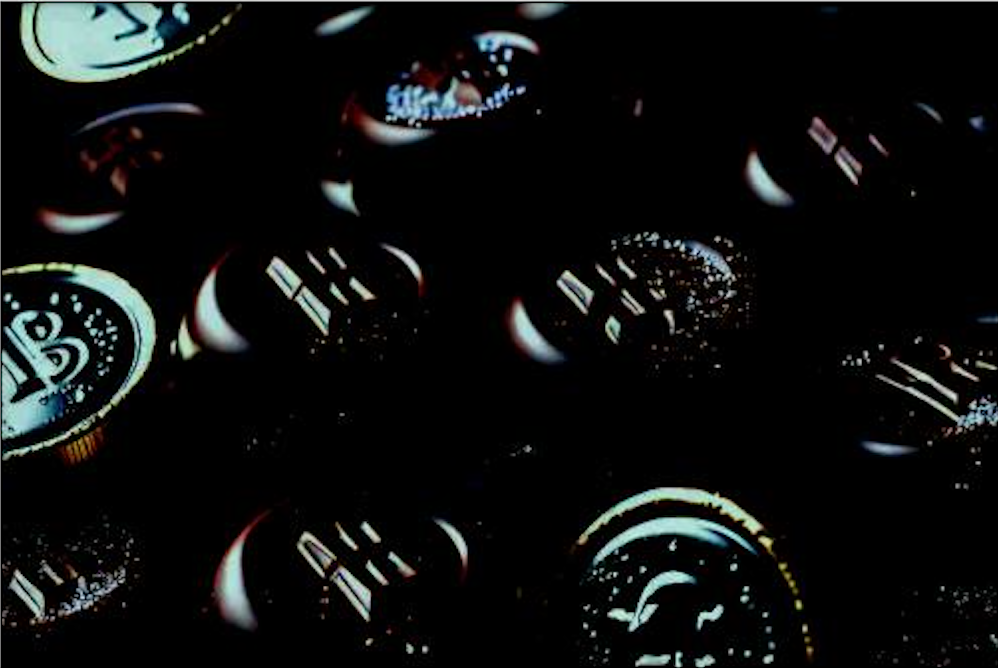
\includegraphics[width=.8\linewidth]{normalized-example}
  \caption{Normalized image example.}
\end{subfigure}
\caption{Examples of data preprocessing steps.}
\label{fig:example-preprocessing-steps}
\end{figure}

\section{Model Training}

Each model in this study was trained using specific hyperparameter configurations suited to its architecture and classification task. For all deep learning models, early stopping was applied based on validation loss with a patience of 10 epochs to prevent overfitting. The best-performing model on the validation set was preserved for final evaluation. A summary of the key training hyperparameters is provided in Table~\ref{tab:training-hyperparameters}.

\textbf{ResNet50} was trained for 100 epochs with a batch size of 16 and input image size of $224 \times 224$. Binary cross-entropy (BCE) loss was used for binary classification tasks and categorical cross-entropy (CCE) for multi-class classification. The Adam optimizer was employed with an initial learning rate of $1 \times 10^{-3}$, along with weight decay of $1 \times 10^{-5}$. A 1-cycle learning rate scheduler was used to adjust the learning rate dynamically over the epochs.

\textbf{EfficientNet} was trained for 100 epochs using a batch size of 16 and input size of $224 \times 224$. For binary classification, the Nesterov momentum variant of Adam (NAdam) was used with a learning rate of $2 \times 10^{-3}$, zero weight decay, and a momentum decay of 0.004. For multi-class classification, the Adam optimizer with an initial learning rate of $1 \times 10^{-3}$ was used. In both cases, the model’s fully connected layer was modified to a linear layer, where the number of output features matched the number of classes.

\textbf{Vision Transformer (ViT)} was trained for 100 epochs with a batch size of 16 and input image size of $224 \times 224$. The Adam optimizer with a learning rate of $2 \times 10^{-5}$ was used, and loss functions were selected according to the classification task (BCE for binary, CCE for multi-class).

\textbf{YOLOv11} was trained for 100 epochs with a batch size of 16 and input image size of $224 \times 224$. SGD was used as the optimizer with an initial learning rate of 0.01, momentum of 0.9, and weight decay of 0.0005. Binary cross-entropy and categorical cross-entropy were used for binary and multi-class classification, respectively.

\textbf{OpenCLIP-based models}: When using OpenCLIP as a feature encoder followed by classical machine learning classifiers, embeddings were extracted from resized input images ($224 \times 224$), and classifiers (e.g., logistic regression, SVM, KNN) were trained on these features. These training processes were straightforward and executed on CPU. In contrast, zero-shot classification with OpenCLIP and Moondream did not involve training on the dataset. Instead, classification was performed by measuring the cosine similarity between image and text embeddings, enabling inference without fine-tuning.

All training experiments were conducted on an NVIDIA RTX 4090 GPU with 16 GB VRAM (10 GB available).

%! Author = zhiweizhang
%! Date = 10.06.25

% Preamble
\begin{table}[ht]
\centering
\resizebox{\textwidth}{!}{
\begin{threeparttable}

\begin{tabular}{lcccccc}
\toprule
\textbf{Model}                  & \textbf{Epochs} & \textbf{Batch Size} & \textbf{Input Size} & \textbf{Loss Function} & \textbf{Optimizer} & \textbf{Learning Rate}  \\
\midrule
ResNet-34                       & 100             & 48                  & 224×224             & BCE/CCE\tnote{1}       & Adam               & 1e-3                    \\
EfficientNet-b2 (binary)        & 100             & 48                  & 224×224             & BCE                    & Nadam              & 2e-3                    \\
EfficientNet-b2 (multi)         & 100             & 48                  & 224×224             & CCE                    & Adam               & 1e-3                    \\
ViT                             & 100             & 48                  & 224×224             & BCE/CCE                & Adam               & 2e-5                    \\
YOLOv11                         & 100             & 48                  & 224×224             & BCE/CCE                & SGD                & 0.01                    \\
OpenCLIP + ML                   & –               & –                   & 224×224             & –                      & –                  & –                       \\
Zero-shot (OpenCLIP, Moondream)\tnote{2} & –               & –                   & –                   & –                      & –                  & –                       \\
\bottomrule
\end{tabular}

\smallskip\footnotesize
\begin{tablenotes}
    \item[1] BCE = Binary Cross-Entropy, CCE = Categorical Cross-Entropy.\vfill
    \item[2] Zero-shot models are not trained on the dataset; they use pretrained weights and inference directly.

\end{tablenotes}
\end{threeparttable}
}
\caption{Summary of training hyperparameters used for each model.}
\label{tab:training-hyperparameters}
\end{table}

\begin{figure}[ht]
    \centering
    \begin{tikzpicture}
        \pie[text=legend, radius=3,
            color={blue!60, red!70}] % 99435 + 2338
            {97.7/Non-Nazi, 2.3/Nazi}
    \end{tikzpicture}
    \caption{Pie chart showing binary classification dataset distribution.}
    \label{fig:binary-dataset-pie}
\end{figure}



\begin{figure}[ht]
    \centering
    \begin{tikzpicture}
        \begin{axis}[
            xbar,
            bar width=10pt,
            width=\textwidth,
            height=9cm,
            xlabel={Number of Images},
            symbolic y coords={
                swastika,
                siegrune,
                ss\_skull,
                hitler,
                neo-nazi,
                black\_sun,
                happy\_merchant,
                wolfsangel,
                broken\_sun\_cross,
                british\_union\_of\_fascist,
                sturmabteilung\_emblem,
                hitler\_salute,
                judenstern
            },
            ytick=data,
            yticklabels={
                Swastika,
                Siegrune,
                SS Skull,
                Hitler,
                Neo-Nazi,
                Black Sun,
                Happy Merchant,
                Wolfsangel,
                Broken Sun Cross,
                British Union of Fascist,
                Sturmabteilung Emblem,
                Hitler Salute,
                Judenstern
            },
            xmin=0,
            xmax=1200,
            nodes near coords,
            nodes near coords align={horizontal},
            enlarge y limits=0.1,
            grid=major,
            bar shift=0pt,
            ]

            % bars with color coding
            \addplot[fill=red!70] coordinates {(1070,swastika)};
            \addplot[fill=orange!70] coordinates {(311,siegrune)};
            \addplot[fill=green!70] coordinates {(257,ss\_skull)};
            \addplot[fill=purple!70] coordinates {(228,hitler)};
            \addplot[fill=yellow!70] coordinates {(188,neo-nazi)};
            \addplot[fill=cyan!70] coordinates {(152,black\_sun)};
            \addplot[fill=brown!70] coordinates {(39,happy\_merchant)};
            \addplot[fill=gray!70] coordinates {(38,wolfsangel)};
            \addplot[fill=magenta!70] coordinates {(21,broken\_sun\_cross)};
            \addplot[fill=teal!70] coordinates {(13,british\_union\_of\_fascist)};
            \addplot[fill=pink!70] coordinates {(11,sturmabteilung\_emblem)};
            \addplot[fill=lime!70] coordinates {(6,hitler\_salute)};
            \addplot[fill=olive!70] coordinates {(4,judenstern)};
        \end{axis}
    \end{tikzpicture}
    \caption{Dataset distribution of the multi-class classification task.}
    \label{fig:multi-class-dataset-distribution}
\end{figure}

%! Author = zhiweizhang
%! Date = 10.06.25

\chapter{Results}\label{chapter:results}


\section{Binary Classification Results}

\subsection{Tabular Results}

The results for the binary classification task are summarized in ~\autoref{tab:binary-results}, which reports
accuracy, precision, recall, and F1-score for each evaluated model, \ac{AUC} and \ac{AP} for applicable models.

%! Author = zhiweizhang
%! Date = 10.06.25

\begin{table}[ht]
\centering
\resizebox{\textwidth}{!}{
\begin{tabular}{lccccc}
\toprule
\textbf{Model}                        & \textbf{Accuracy} & \textbf{Precision} & \textbf{Recall} & \textbf{F1-Score} & \textbf{AUC}   \\
\midrule
YOLOv11                               & 0.995             & 0.793              & 0.932           & 0.857             & 0.964          \\
ResNet                                & 0.996             & 0.843              & 0.893           & 0.867             & 0.945          \\
EfficientNet                          & 0.993             & 0.772              & 0.761           & 0.767             & 0.878          \\
ViT                                   & 0.997             & 0.910              & 0.893           & 0.901             & 0.945          \\
Moondream                             & 0.718             & 0.046              & 1.000           & 0.088             & 0.857          \\
OpenCLIP                              & 0.314             & 0.013              & 0.639           & 0.025             & 0.474          \\
OpenCLIP + Logistic Regression        & 0.996             & 0.923              & 0.882           & 0.902             & 0.940          \\
OpenCLIP + SGDClassifier              & 0.996             & 0.924              & 0.880           & 0.901             & 0.939          \\
OpenCLIP + KNeighborsClassifier       & 0.996             & 0.895              & \textbf{0.936}  & 0.915             & \textbf{0.966} \\
OpenCLIP + SVC                        & \textbf{0.997}    & 0.948              & 0.929           & \textbf{0.939}    & 0.964          \\
OpenCLIP + DecisionTreeClassifier     & 0.987             & 0.674              & 0.742           & 0.706             & 0.867          \\
OpenCLIP + BaggingClassifier          & 0.989             & 0.744              & 0.717           & 0.730             & 0.856          \\
OpenCLIP + AdaBoostClassifier         & 0.994             & 0.901              & 0.791           & 0.842             & 0.894          \\
OpenCLIP + GradientBoostingClassifier & 0.993             & 0.879              & 0.801           & 0.838             & 0.899          \\
OpenCLIP + RandomForestClassifier     & 0.981             & \textbf{0.983}     & 0.097           & 0.177             & 0.548          \\
OpenCLIP + VotingClassifier           & 0.996             & 0.945              & 0.873           & 0.908             & 0.936          \\
\bottomrule
\end{tabular}
}
  \caption{Binary classification performance across different models. The best scores for each metric are highlighted in bold.}
\label{tab:binary-results}
\end{table}


\subsection{Visual Comparison}

To facilitate a clear visual comparison of model performance on the binary classification task, bar plots were
generated for all selected models, including \ac{YOLO}, \ac{ResNet}, EfficientNet, \ac{ViT}, Moondream, OpenCLIP, and
OpenCLIP combined with \ac{SVC}.

~\autoref{fig:model-accuracy}, \autoref{fig:model-precision}, \autoref{fig:model-recall}, and
\autoref{fig:model-f1-score} depict the performance metrics, with the y-axis of each figure representing a metric of
the classification results. These visualizations highlight trade-offs among models and assist in identifying
the most effective architectures.

For binary classification, \ac{ViT}, \ac{YOLO}, and OpenCLIP-based models paired with classical
classifiers—particularly \ac{SVC} and KNeighborsClassifier—demonstrated superior performance. Specifically, \ac{ViT} and
OpenCLIP + \ac{SVC} achieved the highest F1-scores of 0.901 and 0.939, respectively. Conversely, Moondream and the
base OpenCLIP model exhibited comparatively lower effectiveness.

Notably, \textbf{Moondream} significantly underperformed across all metrics. This likely stems from its
architectural and training objectives: Moondream is a vision-language model optimized for tasks such as caption
generation and dialogue, rather than image classification. Its decoding component, aligned with safety mechanisms,
may intentionally suppress or censor content related to hate symbols—including omitting, paraphrasing, or
generalizing textual outputs when prompted about Nazi iconography. Such behavior undermines reliability in
downstream classification tasks where semantic precision is essential. Furthermore, its visual encoder may lack the
granularity necessary to distinguish between visually similar yet semantically distinct symbols—such as swastikas
versus unrelated geometric designs.

Similarly, the \textbf{OpenCLIP model alone} showed limited classification capability. As OpenCLIP is trained
primarily for contrastive image-text retrieval, its raw embeddings—when used without fine-tuning or a dedicated
classifier—may not form well-separated decision boundaries between symbol classes. However, when paired with
classical classifiers such as \textbf{SVC} or \textbf{KNN}, performance improved substantially. This suggests that
while OpenCLIP embeddings capture semantically meaningful image features, they require further downstream
supervision to align with fine-grained classification objectives.

Potential reasons behind the varying performance of different models, including these observations, are further
examined in the ~\autofullref{chapter:discussion-and-analysis}.

%! Author = zhiweizhang
%! Date = 11.06.25

% Preamble
\begin{figure}[ht]
    \centering
    \begin{tikzpicture}
        \begin{axis}[
            ybar,
            bar width=19pt,
            width=\textwidth,
            height=8cm,
            enlarge x limits=0.4,
            ylabel={Accuracy (\%)},
            symbolic x coords={Binary, Multi-class},
            xtick=data,
            ymin=0.0, ymax=110.0,
            nodes near coords,
            nodes near coords align={vertical},
            major x tick style = transparent,
            legend style={
                at={(0.5,-0.2)},
                anchor=north,
                legend columns=3,
                /tikz/every even column/.append style={column sep=0.3cm}
            }
        ]
        \addplot+[style={fill=blue!60}]      coordinates {(Binary, 85.7) (Multi-class, 83.3)};
        \addplot+[style={fill=yellow!60}]    coordinates {(Binary, 86.7) (Multi-class, 81.0)};
        \addplot+[style={fill=brown!50}]     coordinates {(Binary, 76.7) (Multi-class, 70.9)};
        \addplot+[style={fill=purple!50}]    coordinates {(Binary, 90.1) (Multi-class, 79.0)};
        \addplot+[style={fill=orange!70}]    coordinates {(Binary, 26.5) (Multi-class, 35.5)};
        \addplot+[style={fill=red!60}]       coordinates {(Binary, 2.5) (Multi-class, 26.5)};
        \addplot+[style={fill=green!60}]     coordinates {(Binary, 93.9) (Multi-class, 78.4)};
        \legend{
            YOLO,
            ResNet,
            EfficientNet,
            ViT,
            Moondream,
            OpenCLIP,
            OpenCLIP+SVC
        }
        \end{axis}
    \end{tikzpicture}
    \caption{Comparison of F1-score values for all models on binary (left) and multi-class (right) classification tasks.}
    \label{fig:model-f1-score}
\end{figure}
%! Author = zhiweizhang
%! Date = 11.06.25

% Preamble
\begin{figure}[ht]
    \centering
    \begin{tikzpicture}
        \begin{axis}[
            ybar,
            bar width=19pt,
            width=\textwidth,
            height=8cm,
            enlarge x limits=0.4,
            ylabel={Accuracy (\%)},
            symbolic x coords={Binary, Multi-class},
            xtick=data,
            ymin=0.0, ymax=110.0,
            nodes near coords,
            nodes near coords align={vertical},
            major x tick style = transparent,
            legend style={
                at={(0.5,-0.2)},
                anchor=north,
                legend columns=3,
                /tikz/every even column/.append style={column sep=0.3cm}
            }
        ]
        \addplot+[style={fill=blue!60}]      coordinates {(Binary, 99.5) (Multi-class, 88.4)};
        \addplot+[style={fill=yellow!60}]    coordinates {(Binary, 99.6) (Multi-class, 87.9)};
        \addplot+[style={fill=brown!50}]     coordinates {(Binary, 90.3) (Multi-class, 80.1)};
        \addplot+[style={fill=purple!50}]    coordinates {(Binary, 99.7) (Multi-class, 87.6)};
        \addplot+[style={fill=orange!70}]    coordinates {(Binary, 92.4) (Multi-class, 60.8)};
        \addplot+[style={fill=red!60}]       coordinates {(Binary, 31.4) (Multi-class, 27.4)};
        \addplot+[style={fill=green!60}]     coordinates {(Binary, 99.7) (Multi-class, 87.6)};
        \legend{
            YOLO,
            ResNet,
            EfficientNet,
            ViT,
            Moondream,
            OpenCLIP,
            OpenCLIP+SVC
        }
        \end{axis}
    \end{tikzpicture}
    \caption{Comparison of accuracy scores for all models on binary (left) and multi-class (right) classification tasks.}
    \label{fig:model-accuracy}
\end{figure}
%! Author = zhiweizhang
%! Date = 11.06.25

% Preamble
\begin{figure}[ht]
    \centering
    \begin{tikzpicture}
        \begin{axis}[
            ybar,
            bar width=19pt,
            width=\textwidth,
            height=8cm,
            enlarge x limits=0.4,
            ylabel={Accuracy (\%)},
            symbolic x coords={Binary, Multi-class},
            xtick=data,
            ymin=0.0, ymax=110.0,
            nodes near coords,
            nodes near coords align={vertical},
            major x tick style = transparent,
            legend style={
                at={(0.5,-0.2)},
                anchor=north,
                legend columns=3,
                /tikz/every even column/.append style={column sep=0.3cm}
            }
        ]
        \addplot+[style={fill=blue!60}]      coordinates {(Binary, 79.3) (Multi-class, 86.5)};
        \addplot+[style={fill=yellow!60}]    coordinates {(Binary, 61.9) (Multi-class, 73.6)};
        \addplot+[style={fill=brown!50}]     coordinates {(Binary, 80.5) (Multi-class, 71.0)};
        \addplot+[style={fill=purple!50}]    coordinates {(Binary, 87.0) (Multi-class, 83.3)};
        \addplot+[style={fill=orange!70}]    coordinates {(Binary, 4.6) (Multi-class, 41.2)};
        \addplot+[style={fill=red!60}]       coordinates {(Binary, 1.3) (Multi-class, 35.4)};
        \addplot+[style={fill=green!60}]     coordinates {(Binary, 94.8) (Multi-class, 72.3)};
        \legend{
            YOLOv11,
            ResNet50,
            EfficientNetB2,
            ViT,
            Moondream,
            OpenCLIP,
            OpenCLIP+SVC
        }
        \end{axis}
    \end{tikzpicture}
    \caption{Classification precision of selected models for binary and multi-class tasks.}
    \label{fig:model-precision}
\end{figure}
%! Author = zhiweizhang
%! Date = 11.06.25

% Preamble
\begin{figure}[ht]
    \centering
    \begin{tikzpicture}
        \begin{axis}[
            ybar,
            bar width=19pt,
            width=\textwidth,
            height=8cm,
            enlarge x limits=0.4,
            ylabel={Accuracy (\%)},
            symbolic x coords={Binary, Multi-class},
            xtick=data,
            ymin=0.0, ymax=110.0,
            nodes near coords,
            nodes near coords align={vertical},
            major x tick style = transparent,
            legend style={
                at={(0.5,-0.2)},
                anchor=north,
                legend columns=3,
                /tikz/every even column/.append style={column sep=0.3cm}
            }
        ]
        \addplot+[style={fill=blue!60}]      coordinates {(Binary, 93.2) (Multi-class, 81.8)};
        \addplot+[style={fill=yellow!60}]    coordinates {(Binary, 63.4) (Multi-class, 65.5)};
        \addplot+[style={fill=brown!50}]     coordinates {(Binary, 79.9) (Multi-class, 69.7)};
        \addplot+[style={fill=purple!50}]    coordinates {(Binary, 91.2) (Multi-class, 77.5)};
        \addplot+[style={fill=orange!70}]    coordinates {(Binary, 100.0) (Multi-class, 60.1)};
        \addplot+[style={fill=red!60}]       coordinates {(Binary, 63.9) (Multi-class, 41.3)};
        \addplot+[style={fill=green!60}]     coordinates {(Binary, 92.9) (Multi-class, 59.3)};
        \legend{
            YOLOv11,
            ResNet50,
            EfficientNetB2,
            ViT,
            Moondream,
            OpenCLIP,
            OpenCLIP+SVC
        }
        \end{axis}
    \end{tikzpicture}
    \caption{Comparison of recall scores for all models on binary (left) and multi-class (right) classification tasks.}
    \label{fig:model-recall}
\end{figure}
\newpage

\subsection{Confusion Matrices}

Confusion matrices for the binary classification task are shown in~\autoref{fig:confusion-matrix-binary}. Each
matrix represents a model trained to distinguish images as either \textbf{Nazi} or \textbf{Non-Nazi}.

The evaluated models include \ac{YOLO}, EfficientNet, \ac{ResNet}, \ac{ViT}, and an OpenCLIP encoder paired with a
support vector classifier (SVC). These matrices visualize each model's prediction distribution by presenting true
positives, true negatives, false positives, and false negatives.

In general, most models achieved strong diagonal dominance, indicating successful classification of both Nazi and
non-Nazi symbols. Notably:

\begin{itemize}
\item \textbf{YOLO} and \textbf{EfficientNet} achieved relatively balanced true positive and true negative counts,
reflecting consistent performance across both classes.
\item \textbf{ResNet} and \textbf{ViT} also performed reliably, with lower false positive rates, suggesting a
cautious approach that reduces mislabeling benign symbols as Nazi-related.
\item The \textbf{OpenCLIP+SVC} configuration showed improved class separation compared to raw OpenCLIP outputs,
confirming the importance of combining feature extractors with downstream classifiers.
\end{itemize}

However, misclassifications still occurred—particularly false negatives, where Nazi symbols were not detected. These
errors highlight the difficulty of classifying visually degraded, ambiguous, or stylistically subtle symbols, which
will be analyzed in depth in ~\autofullref{chapter:discussion-and-analysis}.

%! Author = zhiweizhang
%! Date = 13.06.25

% Preamble
\begin{figure}[ht]
    \begin{subfigure}[b]{0.45\textwidth}
    \centering
        \begin{tikzpicture}
            \begin{axis}[
                width=0.9\textwidth,
                colormap={bluewhite}{color=(white) rgb255=(90,96,191)},
                xlabel=Predicted,
                ylabel=Actual,
                xticklabels={Non-Nazi, Nazi}, % changed
                xtick={0,...,1}, % changed
                xtick style={draw=none},
                yticklabels={Non-Nazi, Nazi}, % changed
                ytick={0,...,1}, % changed
                ytick style={draw=none},
                enlargelimits=false,
                colorbar,
                point meta min=0,
                point meta max=200,
                xticklabel style={
                  text width=1cm,align=center
                },
                yticklabel style={
                  text width=1cm,align=center
                },
                nodes near coords={\pgfmathprintnumber\pgfplotspointmeta},
                nodes near coords style={
                    yshift=-7pt
                },
            ]
                \addplot[
                    matrix plot,
                    mesh/cols=2, % changed
                    point meta=explicit,
                    draw=gray
                ] table [meta=C, x=x, y=y, col sep=comma] {data/yolo-binary-confusion-matrix-data.csv};
            \end{axis}
        \end{tikzpicture}
        \caption{Confusion matrix of YOLO.}\label{fig:yolo-confusion-matrix-binary}
    \end{subfigure}
    \hfill
    \begin{subfigure}[b]{0.45\textwidth}
    \centering
        \begin{tikzpicture}
            \begin{axis}[
                width=0.9\textwidth,
                colormap={bluewhite}{color=(white) rgb255=(90,96,191)},
                xlabel=Predicted,
                ylabel=Actual,
                xticklabels={Non-Nazi, Nazi}, % changed
                xtick={0,...,1}, % changed
                xtick style={draw=none},
                yticklabels={Non-Nazi, Nazi}, % changed
                ytick={0,...,1}, % changed
                ytick style={draw=none},
                enlargelimits=false,
                colorbar,
                point meta min=0,
                point meta max=200,
                xticklabel style={
                  text width=1cm,align=center
                },
                yticklabel style={
                  text width=1cm,align=center
                },
                nodes near coords={\pgfmathprintnumber\pgfplotspointmeta},
                nodes near coords style={
                    yshift=-7pt
                },
            ]
                \addplot[
                    matrix plot,
                    mesh/cols=2, % changed
                    point meta=explicit,
                    draw=gray
                ] table [meta=C, x=x, y=y, col sep=comma] {data/efficientnet-binary-confusion-matrix-data.csv};
            \end{axis}
        \end{tikzpicture}
        \caption{Confusion matrix of EfficientNet.}\label{fig:efficient-confusion-matrix-binary}
    \end{subfigure}
    \hfill
    \begin{subfigure}[b]{0.45\textwidth}
    \centering
        \begin{tikzpicture}
            \begin{axis}[
                width=0.9\textwidth,
                colormap={bluewhite}{color=(white) rgb255=(90,96,191)},
                xlabel=Predicted,
                ylabel=Actual,
                xticklabels={Non-Nazi, Nazi}, % changed
                xtick={0,...,1}, % changed
                xtick style={draw=none},
                yticklabels={Non-Nazi, Nazi}, % changed
                ytick={0,...,1}, % changed
                ytick style={draw=none},
                enlargelimits=false,
                colorbar,
                point meta min=0,
                point meta max=200,
                xticklabel style={
                  text width=1cm,align=center
                },
                yticklabel style={
                  text width=1cm,align=center
                },
                nodes near coords={\pgfmathprintnumber\pgfplotspointmeta},
                nodes near coords style={
                    yshift=-7pt
                },
            ]
                \addplot[
                    matrix plot,
                    mesh/cols=2, % changed
                    point meta=explicit,
                    draw=gray
                ] table [meta=C, x=x, y=y, col sep=comma] {data/openclip_encoder-binary-confusion-matrix-data.csv};
            \end{axis}
        \end{tikzpicture}
        \caption{Confusion matrix of OpenCLIP encoder and SVC.}\label{fig:openclip-encoder-confusion-matrix-binary}
    \end{subfigure}
    \hfill
    \begin{subfigure}[b]{0.45\textwidth}
    \centering
        \begin{tikzpicture}
            \begin{axis}[
                width=0.9\textwidth,
                colormap={bluewhite}{color=(white) rgb255=(90,96,191)},
                xlabel=Predicted,
                ylabel=Actual,
                xticklabels={Non-Nazi, Nazi}, % changed
                xtick={0,...,1}, % changed
                xtick style={draw=none},
                yticklabels={Non-Nazi, Nazi}, % changed
                ytick={0,...,1}, % changed
                ytick style={draw=none},
                enlargelimits=false,
                colorbar,
                point meta min=0,
                point meta max=200,
                xticklabel style={
                  text width=1cm,align=center
                },
                yticklabel style={
                  text width=1cm,align=center
                },
                nodes near coords={\pgfmathprintnumber\pgfplotspointmeta},
                nodes near coords style={
                    yshift=-7pt
                },
            ]
                \addplot[
                    matrix plot,
                    mesh/cols=2, % changed
                    point meta=explicit,
                    draw=gray
                ] table [meta=C, x=x, y=y, col sep=comma] {data/resnet-binary-confusion-matrix-data.csv};
            \end{axis}
        \end{tikzpicture}
        \caption{Confusion matrix of ResNet.}\label{fig:resnet-encoder-confusion-matrix-binary}
    \end{subfigure}
    \hfill
    \begin{subfigure}[b]{0.45\textwidth}
    \centering
        \begin{tikzpicture}
            \begin{axis}[
                width=0.9\textwidth,
                colormap={bluewhite}{color=(white) rgb255=(90,96,191)},
                xlabel=Predicted,
                ylabel=Actual,
                xticklabels={Non-Nazi, Nazi}, % changed
                xtick={0,...,1}, % changed
                xtick style={draw=none},
                yticklabels={Non-Nazi, Nazi}, % changed
                ytick={0,...,1}, % changed
                ytick style={draw=none},
                enlargelimits=false,
                colorbar,
                point meta min=0,
                point meta max=200,
                xticklabel style={
                  text width=1cm,align=center
                },
                yticklabel style={
                  text width=1cm,align=center
                },
                nodes near coords={\pgfmathprintnumber\pgfplotspointmeta},
                nodes near coords style={
                    yshift=-7pt
                },
            ]
                \addplot[
                    matrix plot,
                    mesh/cols=2, % changed
                    point meta=explicit,
                    draw=gray
                ] table [meta=C, x=x, y=y, col sep=comma] {data/vit-binary-confusion-matrix-data.csv};
            \end{axis}
        \end{tikzpicture}
        \caption{Confusion matrix of ViT.}\label{fig:vit-encoder-confusion-matrix-binary}
    \end{subfigure}

    \caption{Confusion matrices illustrating classification results of the binary task for each evaluated model. The matrices display true positive, true negative, false positive, and false negative counts for the classes “Nazi” and “Non-Nazi.”}
    \label{fig:confusion-matrix-binary}
\end{figure}

\subsection{Receiver Operating Characteristic (ROC) and Precision-Recall (PR) Curves}

To further characterize model performance under class imbalance, \ac{ROC} and \ac{PR} curves were plotted for the
binary classification task.

~\autoref{fig:roc-curve} illustrates the \ac{ROC} curves, demonstrating the trade-off between true positive rate and
false positive rate across different thresholds. The \ac{AUC} values reported in ~\autoref{tab:binary-results}
correspond with the visual trends observed. Most models exhibit near-perfect AUC scores ($\geq$0.998), indicating strong
overall separability between Nazi and Non-Nazi classes.

~\autoref{fig:pr-curve} presents the \ac{PR} curves, which are particularly informative when evaluating classifiers
under imbalanced conditions. The area under the \ac{PR} curve (\ac{AP}) complements the \ac{AUC-ROC},
emphasizing each model's ability to retrieve relevant positive samples effectively. Models such as OpenCLIP +
Logistic Regression (\ac{AP} = 0.964), \ac{ViT} (\ac{AP} = 0.962), and OpenCLIP + SVC (unreported \ac{AP} but high F1)
demonstrate particularly strong precision-recall trade-offs. In contrast, models like EfficientNet and
DecisionTreeClassifier show notably lower AP scores (0.780 and 0.625 respectively), reflecting limitations in
correctly retrieving positive instances under imbalance.

These curves and scores provide a nuanced view of classification confidence and retrieval quality beyond accuracy,
particularly important in safety-critical applications where false positives or false negatives may carry different risks.

\begin{figure}[ht]
  \centering
  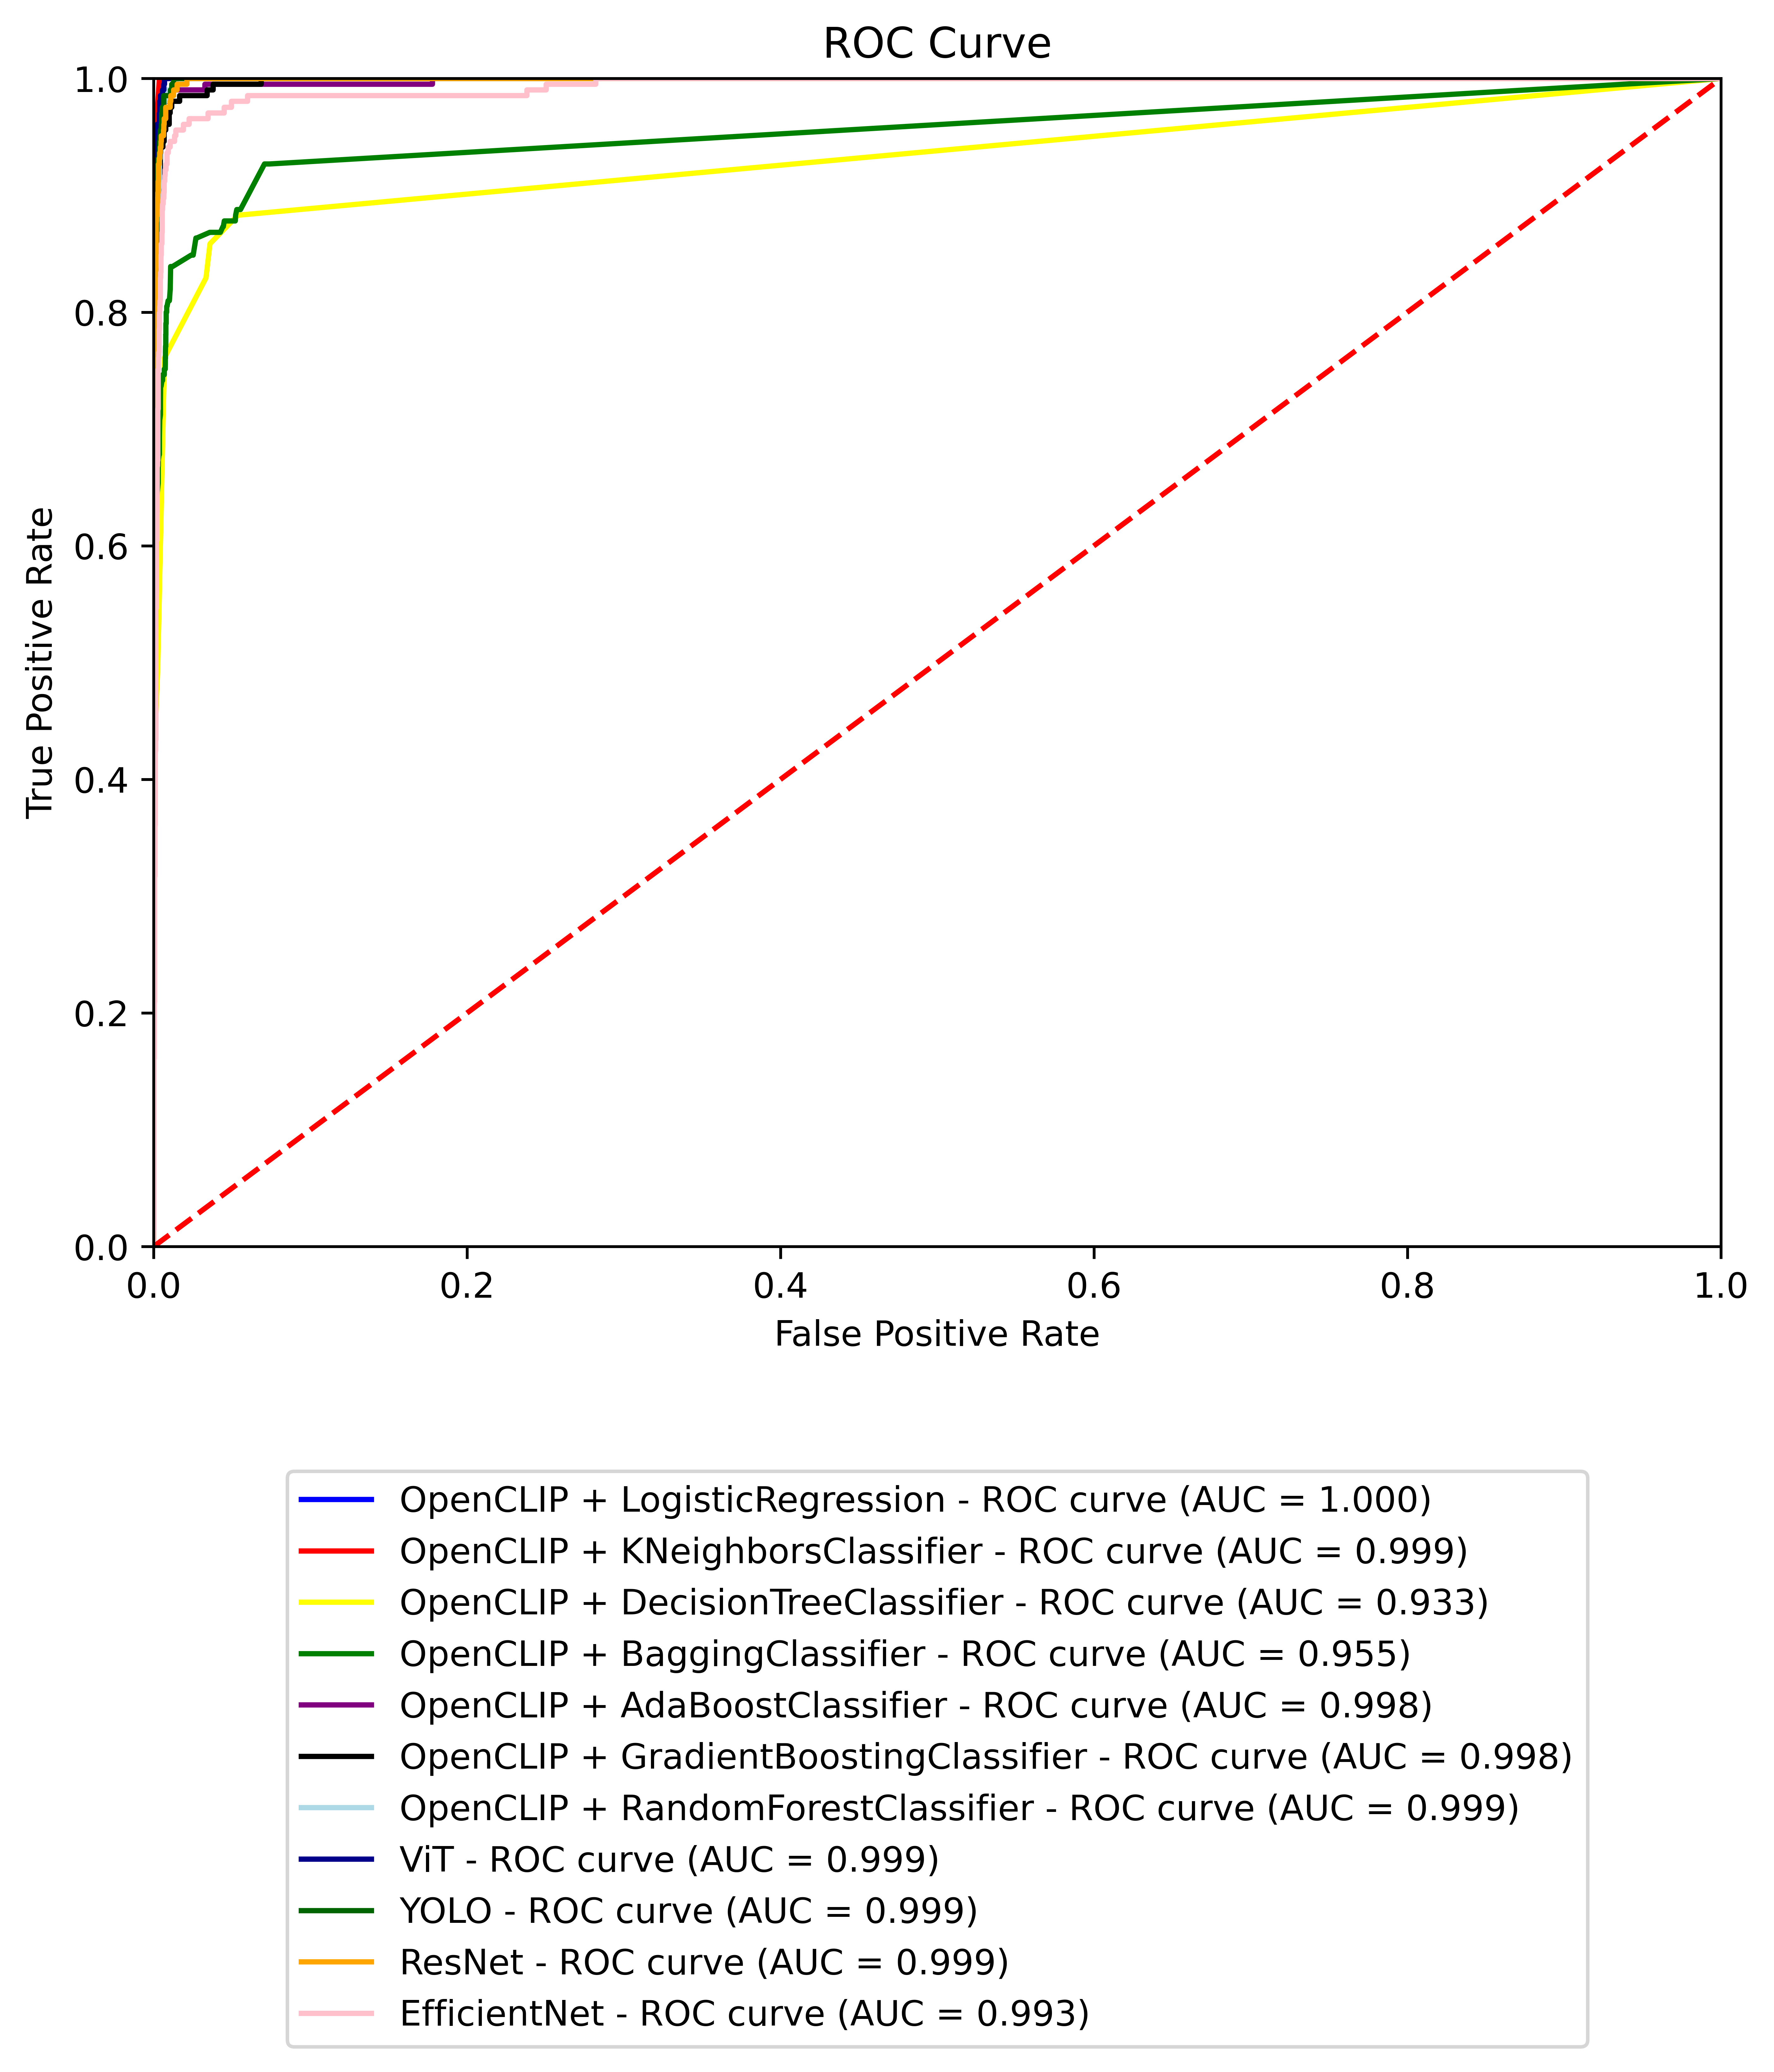
\includegraphics[width=0.8\textwidth]{figures/ROC}
  \caption{Receiver Operating Characteristic (ROC) curves for all models on the binary classification task, depicting the trade-off between true positive rate and false positive rate across classification thresholds.}
  \label{fig:roc-curve}
\end{figure}

\begin{figure}[ht]
  \centering
  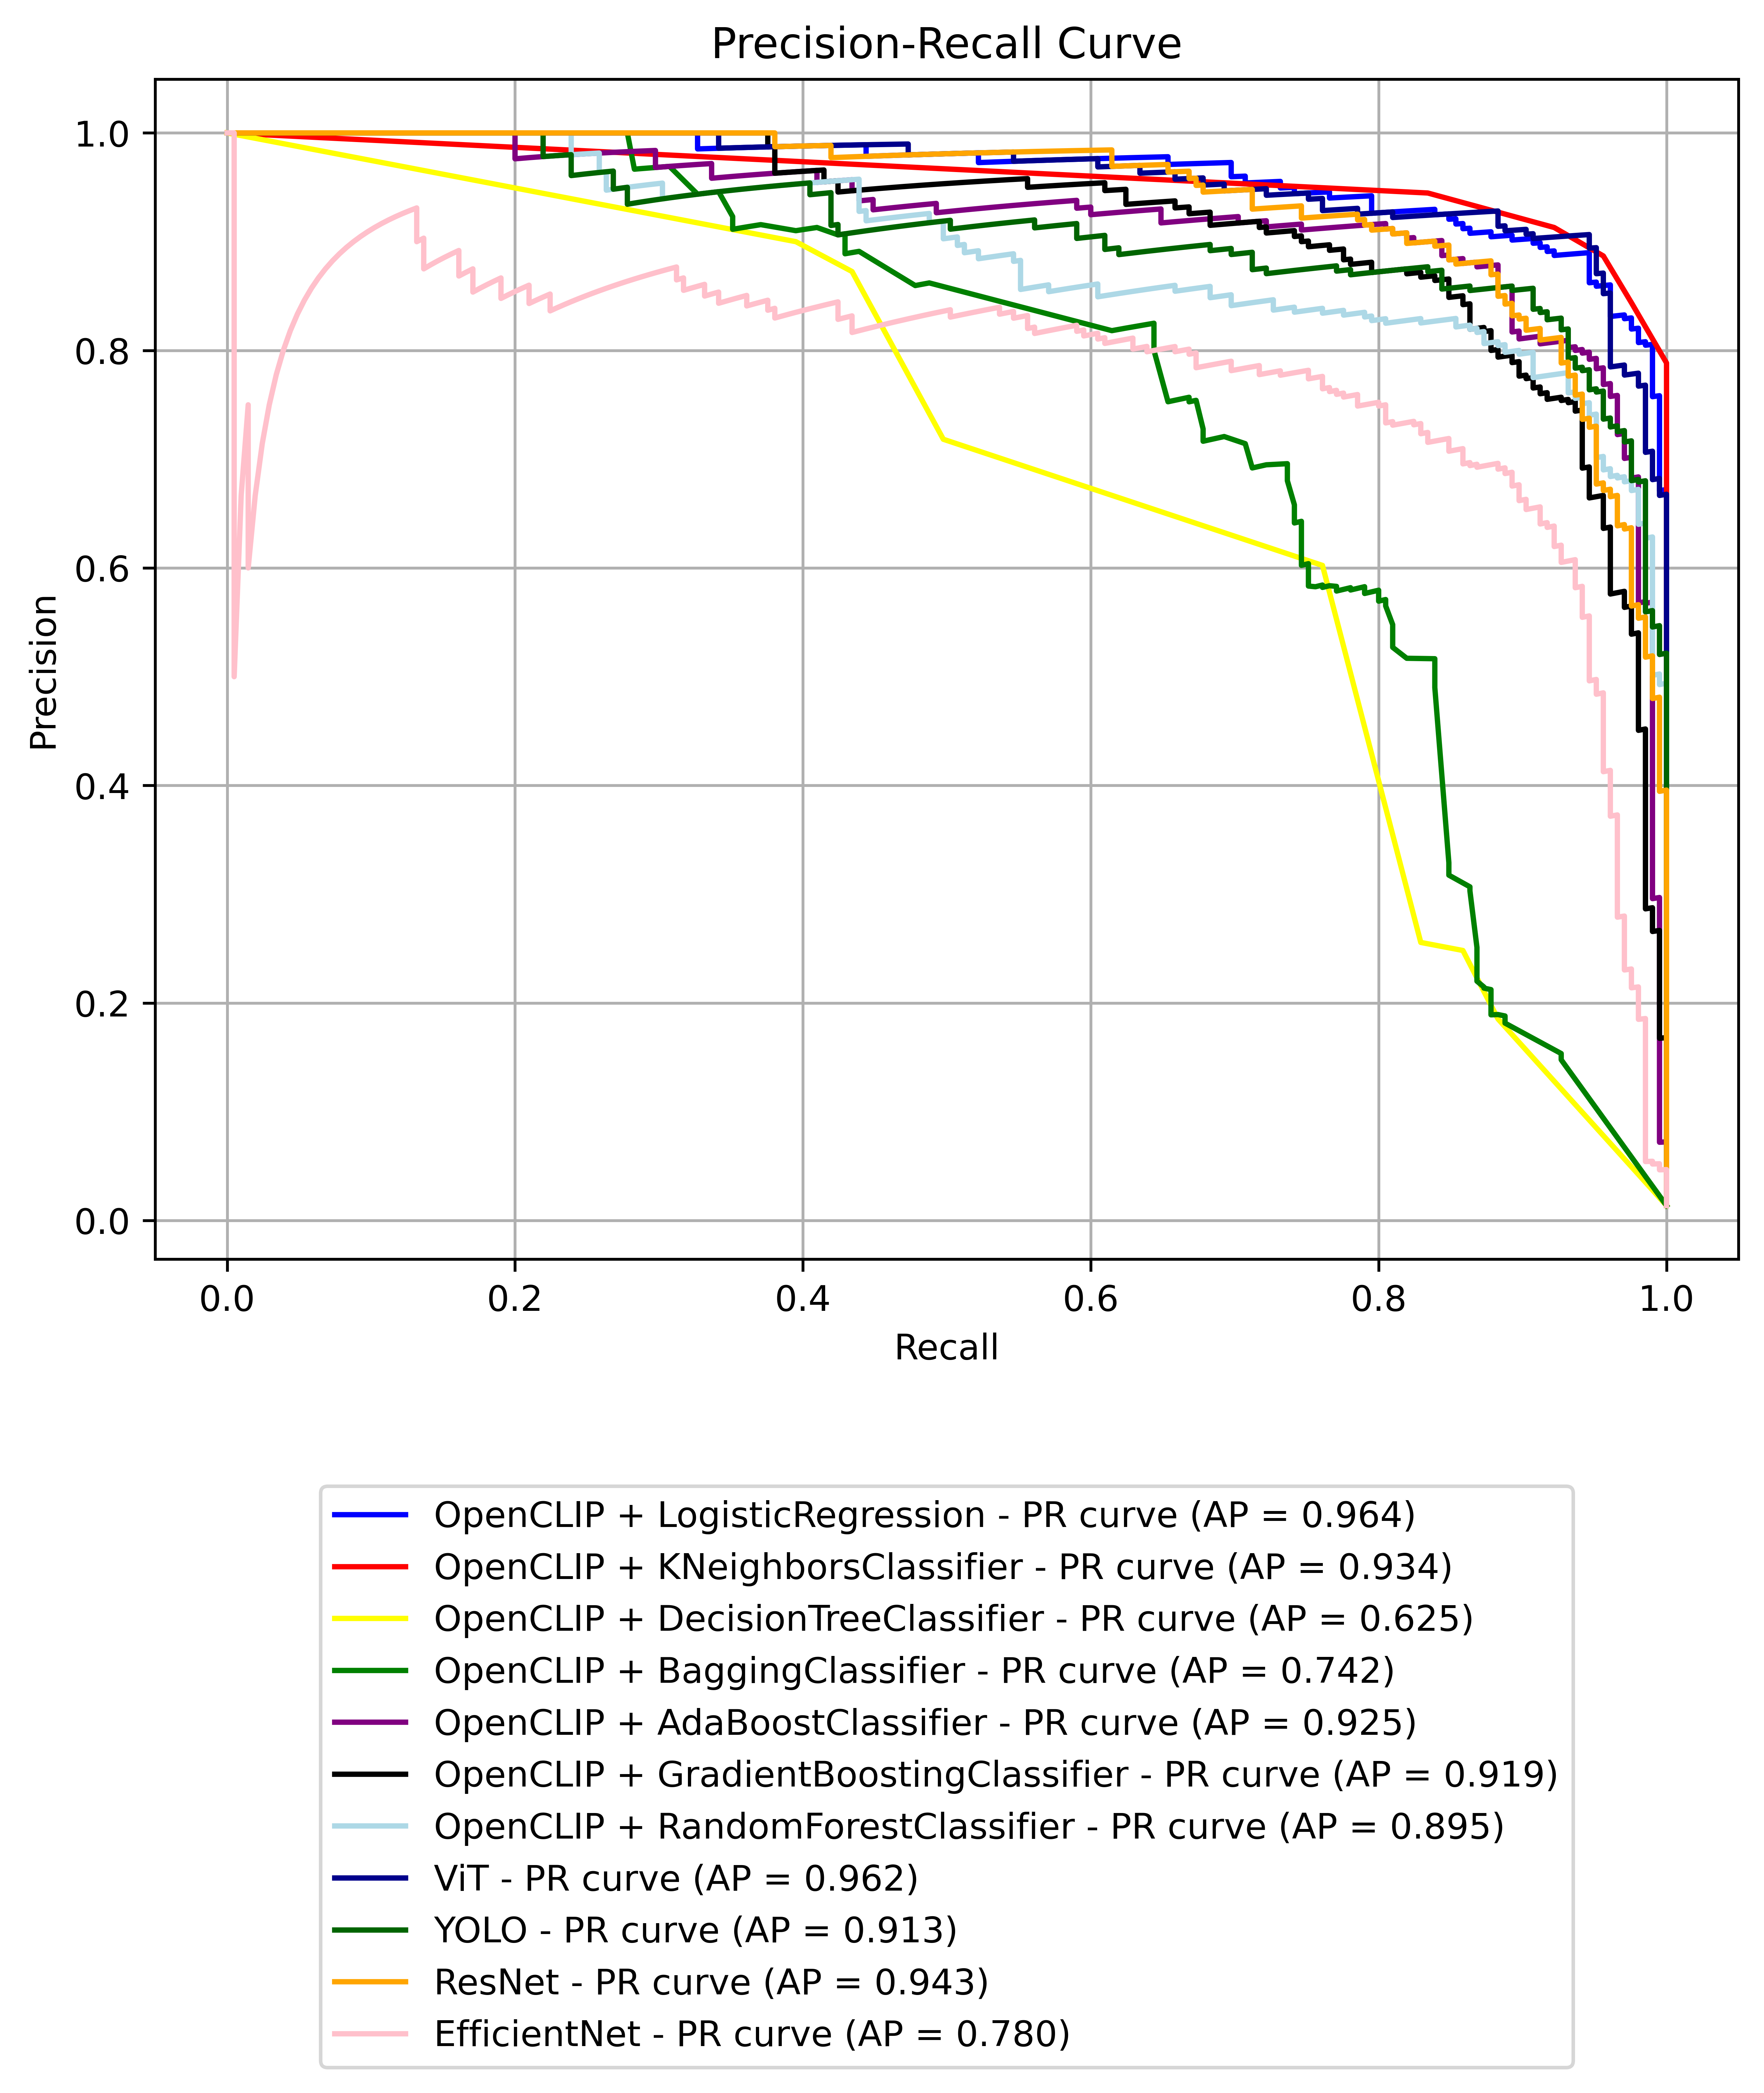
\includegraphics[width=0.8\textwidth]{figures/PR}
  \caption{Precision-Recall (PR) curves for all models on the binary classification task, highlighting model performance under class imbalance conditions.}
  \label{fig:pr-curve}
\end{figure}

\subsection{Reduced-Symbol Set Experiment}

To further evaluate model robustness, an additional experiment was conducted using a reduced set of Nazi symbols
from the original dataset. This subset included the three most visually distinct symbols: the \textit{SS Skull},
\textit{Siegrune}, and \textit{Swastika}.

The results of this reduced-symbol experiment are presented in ~\autoref{tab:binary-reduced-symbols-result},
indicating the models' performance when focusing on a smaller, more visually distinct set of classes.

%! Author = zhiweizhang
%! Date = 10.06.25

\begin{table}[ht]
  \centering
  \resizebox{\textwidth}{!}{
    \begin{tabular}{lccccc}
    \toprule
    \textbf{Model}                        & \textbf{Accuracy} & \textbf{Precision} & \textbf{Recall} & \textbf{F1-Score} \\
    \midrule
    YOLO                                  & 0.994             & 0.792              & 0.568           & 0.661             \\
    ResNet                                & 0.996             & 0.798              & 0.932           & 0.860             \\
    EfficientNet                          & 0.987             & 0.667              & 0.744           & 0.703             \\
    ViT                                   & \textbf{0.998}    & 0.972              & 0.926           & \textbf{0.948}    \\
    Moondream                             & 0.996             & 0.840              & 0.851           & 0.846             \\
    OpenCLIP                              & 0.864             & 0.025              & 0.338           & 0.047             \\
    OpenCLIP + Logistic Regression        & 0.996             & 0.917              & 0.835           & 0.874             \\
    OpenCLIP + SGDClassifier              & 0.996             & 0.899              & 0.895           & 0.897             \\
    OpenCLIP + KNeighborsClassifier       & \textbf{0.998}    & 0.895              & \textbf{0.989}  & 0.940             \\
    OpenCLIP + SVC                        & \textbf{0.998}    & \textbf{0.973}     & 0.900           & 0.935             \\
    OpenCLIP + DecisionTreeClassifier     & 0.985             & 0.514              & 0.635           & 0.568             \\
    OpenCLIP + BaggingClassifier          & 0.987             & 0.566              & 0.639           & 0.600             \\
    OpenCLIP + AdaBoostClassifier         & 0.994             & 0.869              & 0.742           & 0.800             \\
    OpenCLIP + GradientBoostingClassifier & 0.993             & 0.837              & 0.708           & 0.767             \\
    OpenCLIP + RandomForestClassifier     & 0.988             & 0.959              & 0.209           & 0.344             \\
    OpenCLIP + VotingClassifier           & 0.997             & 0.964              & 0.833           & 0.894             \\
    \bottomrule
    \end{tabular}
  }
  \caption{Binary classification performance across different models on reduced-symbol set. The best scores for each metric are highlighted in bold.}
  \label{tab:binary-reduced-symbols-result}
\end{table}

As expected, reducing the class set to visually distinct symbols improved performance across most models. This
demonstrates the impact of inter-class visual similarity on model accuracy. With fewer symbols and more training
samples per class, models could learn cleaner decision boundaries and avoid confusion between ambiguous or
similar-looking symbols.

Implications of improved results on the reduced symbol set, and their relevance to dataset complexity and model
robustness, are explored in more depth in the ~\autofullref{chapter:discussion-and-analysis}.


\section{Multi-Class Classification Results}

\subsection{Tabular Results}

The multi-class classification results are summarized in ~\autoref{tab:multi-class-results}, reporting
macro-averaged accuracy, precision, recall, and F1-score for each model.

%! Author = zhiweizhang
%! Date = 10.06.25

\begin{table}[ht]
\centering
\resizebox{\textwidth}{!}{
\begin{tabular}{lcccc}
\toprule
\textbf{Model}                        & \textbf{Accuracy (Macro)} & \textbf{Precision (Macro)} & \textbf{Recall (Macro)} & \textbf{F1-score (Macro)} \\
\midrule
YOLOv11                               & \textbf{0.884}            & \textbf{0.865}             & \textbf{0.818}          & \textbf{0.833}            \\
ResNet                                & 0.879                     & 0.850                      & 0.795                   & 0.810                     \\
EfficientNet                          & 0.794                     & 0.710                      & 0.697                   & 0.698                     \\
ViT                                   & 0.876                     & 0.833                      & 0.775                   & 0.790                     \\
Moondream                             & 0.608                     & 0.412                      & 0.601                   & 0.355                     \\
OpenCLIP                              & 0.274                     & 0.354                      & 0.413                   & 0.265                     \\
OpenCLIP + Logistic Regression        & 0.768                     & 0.476                      & 0.390                   & 0.412                     \\
OpenCLIP + SGDClassifier              & 0.799                     & 0.749                      & 0.624                   & 0.632                     \\
OpenCLIP + KNeighborsClassifier       & 0.752                     & 0.598                      & 0.518                   & 0.530                     \\
OpenCLIP + SVC                        & 0.815                     & 0.723                      & 0.593                   & 0.620                     \\
OpenCLIP + DecisionTreeClassifier     & 0.577                     & 0.177                      & 0.160                   & 0.154                     \\
OpenCLIP + BaggingClassifier          & 0.599                     & 0.320                      & 0.179                   & 0.177                     \\
OpenCLIP + AdaBoostClassifier         & 0.648                     & 0.404                      & 0.275                   & 0.305                     \\
OpenCLIP + GradientBoostingClassifier & 0.704                     & 0.444                      & 0.412                   & 0.389                     \\
OpenCLIP + RandomForestClassifier     & 0.583                     & 0.261                      & 0.162                   & 0.161                     \\
OpenCLIP + VotingClassifier           & 0.770                     & 0.481                      & 0.391                   & 0.415                     \\
\bottomrule
\end{tabular}
}
  \caption{Multi-class classification performance across different models. The best scores for each metric are highlighted in bold.}
\label{tab:multi-class-results}
\end{table}

\subsection{Visual Comparison}

~\autoref{fig:model-f1-score} \autoref{fig:model-accuracy}, \autoref{fig:model-precision}, and
\autoref{fig:model-recall} also include the multi-class classification results, presented on the right side of
each plot. These visualizations allow for direct comparison of model effectiveness across multiple symbol classes.

In this setting, \ac{YOLO} consistently outperformed other models across all evaluation metrics, followed closely by
\ac{ResNet} and \ac{ViT}, both of which demonstrated strong and consistent classification performance. Models such as
Moondream and OpenCLIP showed less consistent results across different classes.

\subsection{Confusion Matrices}

Confusion matrices for the multi-class classification task are shown in the figures below. Each matrix corresponds
to a model trained to classify images into one of thirteen symbol categories:

\begin{quote}
\texttt{['Black Sun', 'Flash and circle', 'Broken Sun Cross', 'The Happy Merchant', 'Hitler', 'Nazi salute',
  'Yellow badge', 'neo-Nazi', 'Siegrune', 'SS Skull', 'Sturmabteilung emblem', 'Swastika', 'Wolfsangel']}
\end{quote}

These matrices reveal class-specific performance, highlighting where misclassifications occur and identifying
classes that are frequently confused. Such insights assist in understanding model limitations and potential areas
for improvement.

\begin{itemize}
  \item \textbf{\ac{ResNet}:} Demonstrates strong performance on prominent symbols such as \textit{Swastika} and
  \textit{Siegrune}, with occasional confusion among visually similar classes.
  \item \textbf{\ac{YOLO}:} Achieves high accuracy on frequent classes but struggles with rarer symbols like
  \textit{Nazi salute} and \textit{Broken Sun Cross}. Overall, it has the best performance across all classes.
  \item \textbf{EfficientNet:} Yields balanced performance but exhibits reduced confidence on ambiguous or
  underrepresented categories.
  \item \textbf{\ac{ViT}:} Shows strong recognition for dominant classes, with some misclassifications on less
  frequent symbols.
  \item \textbf{OpenCLIP encoder + \ac{SVC}:} The text-image contrastive learning approach produces reasonable results,
  particularly for \textit{Swastika}, but is sensitive to class imbalance.
\end{itemize}

\input{figures/yolo_confusion_matrix_multiclass}
\input{figures/efficientnet_confusion_matrix_multiclass}
\input{figures/resnet_confusion_matrix_multiclass}
\input{figures/vit_confusion_matrix_multiclass}
%! Author = zhiweizhang
%! Date = 13.06.25

% Preamble
\begin{figure}[ht]
    \centering
    \begin{tikzpicture}
        \begin{axis}[
            colormap={bluewhite}{color=(white) rgb255=(90,96,191)},
            xlabel=Predicted,
            xlabel style={yshift=-10pt},
            ylabel=Actual,
            ylabel style={yshift=10pt},
            xticklabels={
                Black Sun,
                Flash and circle,
                Broken Sun Cross,
                The Happy Merchant,
                Hitler,
                Nazi salute,
                Yellow badge,
                Neo-Nazi,
                Siegrune,
                SS Skull,
                Sturmabteilung emblem,
                Swastika,
                Wolfsangel
            }, % changed
            xtick={0,...,12}, % changed
            xtick style={draw=none},
            yticklabels={
                Black Sun,
                Flash and circle,
                Broken Sun Cross,
                The Happy Merchant,
                Hitler,
                Nazi salute,
                Yellow badge,
                Neo-Nazi,
                Siegrune,
                SS Skull,
                Sturmabteilung emblem,
                Swastika,
                Wolfsangel
            }, % changed
            ytick={0,...,12}, % changed
            ytick style={draw=none},
            enlargelimits=false,
            colorbar,
%            colorbar style={
%              ytick={0, 0.5, 1.0, 1.5},
%              yticklabels={0, 0.5, 1.0, 1.5},
%%              xtick=\empty,
%%              ylabel style={yshift=10pt},
%            },
            point meta min=0,
            point meta max=100,
            xticklabel style={
              rotate=90,
            },
%            yticklabel style={
%              text width=1cm,align=center
%            },
            nodes near coords={\pgfmathprintnumber\pgfplotspointmeta},
            nodes near coords style={
                yshift=-7pt
            },
        ]
            \addplot[
                matrix plot,
                mesh/cols=13, % changed
                point meta=explicit,
                draw=gray
            ] table [meta=C, x=x, y=y, col sep=comma] {data/openclip_encoder-multiclass-confusion-matrix-data.csv};
        \end{axis}
    \end{tikzpicture}
    \caption{Confusion matrix for the binary classification task using OpenCLIP encoder and SVC. The values represent the number of samples in each cell.}
    \label{fig:openclip-encoder-confusion-matrix-multiple}
\end{figure}

Across multi-class results, \textbf{YOLO} stands out as the top performer. Its architecture enables spatial
attention and object localization, making it well-suited to distinguish between overlapping or co-located symbols.
In contrast, \textbf{ViT} and \textbf{ResNet} rely on whole-image representations and struggle more with occlusion
or background noise.

Moondream and vanilla OpenCLIP again performed poorly, reinforcing that general-purpose vision-language models are
not optimal for fine-grained symbol classification—especially without prompt engineering or task-specific tuning.

Detailed analysis and interpretation of multi-class classification challenges and model behaviors are deferred to
the ~\autofullref{chapter:discussion-and-analysis}.
%! Author = zhiweizhang
%! Date = 10.06.25

\chapter{Discussion and Analysis}\label{chapter:discussion-and-analysis}

This chapter reflects critically on the performance of the evaluated models, connecting the empirical results to the
research objectives outlined in ~\autofullref{chapter:introduction}. The primary aim of this thesis was to develop
and compare image classification models capable of accurately recognizing and categorizing Nazi symbols from varied
visual inputs. Through detailed analysis of both binary and multi-class classification results, this chapter
interprets key trends, identifies strengths and limitations of different model families, and discusses the practical
and ethical implications of deploying such systems.

\section{Analysis of Binary Classification Performance}

The results presented in ~\autoref{tab:binary-results} reveal a wide range of performances across different models.
Notably, classical \ac{ML} classifiers leveraging OpenCLIP embeddings consistently ranked among the top
performers. The best overall F1-score (0.939) was achieved by the \textbf{OpenCLIP + ~\ac{SVC}} model, which also
demonstrated high precision (0.948) and recall (0.929). Similarly, the \textbf{OpenCLIP + Logistic Regression}
model achieved the highest ~\ac{AUC} score (1.000) and highest \ac{AP} (0.964), along with a strong recall of 0.882
and an F1-score of 0.902, indicating a solid ability to correctly classify Nazi symbols while minimizing false
negatives.

Among \ac{DL} models, both \textbf{\ac{ViT}} and \textbf{\ac{YOLO}} performed competitively. \ac{ViT} achieved an
F1-score of 0.901, the highest among all standalone neural models, while \ac{YOLO} achieved an F1-score of 0.857 with
a notably high recall of 0.932, highlighting its capacity to correctly classify positive symbol instances.
\ac{ResNet} also performed well, with an F1-score of 0.867, slightly outperforming EfficientNet (0.767).

Anomalously, the \textbf{Moondream} model achieved an exceptionally high recall of 0.995 but suffered from very low
precision (0.153), resulting in a low F1-score of just 0.265. This suggests a strong tendency to overpredict the
Nazi class, leading to a high number of false positives. Similarly, the \textbf{OpenCLIP zero-shot} model performed
poorly, with a low F1-score of 0.025, highlighting the limitations of zero-shot classification without additional
fine-tuning or classifier integration.

Several classical ensemble models also showed robust performance when paired with OpenCLIP embeddings. For instance,
\textbf{OpenCLIP + VotingClassifier} reached an F1-score of 0.908 and precision of 0.945, while
\textbf{OpenCLIP + AdaBoostClassifier} and \textbf{OpenCLIP + GradientBoostingClassifier} achieved F1-scores of
0.842 and 0.838, respectively. However, the \textbf{OpenCLIP + RandomForestClassifier} produced an unusually high
precision (0.983) but very low recall (0.097), resulting in a poor F1-score (0.177), indicating that it was highly
conservative in predicting the Nazi class.

Overall, models that combine OpenCLIP embeddings with classical classifiers—especially \ac{SVC}, KNeighborsClassifier, and
VotingClassifier—outperformed all other approaches in this binary classification task. Nonetheless, end-to-end deep
learning models like \ac{ViT} and \ac{YOLO} remain competitive and demonstrate strong generalization capabilities,
particularly when trained on high-resolution inputs and sufficient labeled data.

\subsection{Binary Classification Confusion Matrix Analysis}

~\autoref{fig:confusion-matrix-binary} presents the confusion matrices for the binary classification task, where the
goal is to distinguish between \textit{Nazi} and \textit{Non-Nazi} images.

The OpenCLIP encoder combined with \ac{SVC} achieves the best overall balance, producing the
highest number of true positives (194) and true negatives (14,802), alongside the lowest false positives (11) and
false negatives (11). This indicates a strong capability to correctly classify Nazi symbols while minimizing
misclassifications.

\ac{YOLO} shows excellent sensitivity, with the second lowest false negative count (14), meaning it rarely misses Nazi
instances, but it has a relatively higher false positive rate (50), which might lead to more false alarms.

\ac{ResNet} also performs well, showing a favorable trade-off between false positives (34) and false negatives (22),
maintaining a good level of accuracy and reliability.

\ac{ViT} provides balanced performance, with moderate false positives (28) and false negatives (18), showing
robustness in both detecting Nazi symbols and correctly rejecting non-Nazi images.

EfficientNet, while demonstrating strong true negative results, has the highest false negatives (49), indicating
that it misses more Nazi cases compared to the other models, which might limit its applicability when recall is critical.

Overall, these confusion matrices confirm that the OpenCLIP + \ac{SVC} approach is the most effective for binary
classification in this context, offering a strong balance between precision and recall essential for sensitive
symbol classification.

\subsection{Binary Classification \ac{ROC} and \ac{PR} Curve Analysis}

The \ac{ROC} curve results indicate that most models achieved excellent discriminative ability in the binary
classification task, with several models reaching near-perfect \ac{AUC} values close to 1.0. Notably, OpenCLIP combined
with \ac{LR}, KNeighborsClassifier, and Random Forest classifiers, along with \ac{ViT}, \ac{YOLO},
and \ac{ResNet}, all demonstrated near-identical, near-optimal \ac{ROC} performance (\ac{AUC} $\approx$ 1.000),
suggesting their strong capacity to separate Nazi and Non-Nazi classes.

Ensemble methods such as AdaBoost and Gradient Boosting classifiers paired with OpenCLIP embeddings also performed
robustly (\ac{AUC} $\approx$ 0.998), while EfficientNet’s slightly lower \ac{AUC} of 0.993 still represents a high-quality
classification boundary. Bagging and Decision Tree classifiers showed comparatively lower \ac{AUC}s (0.955 and 0.933),
indicating reduced robustness and potential susceptibility to misclassification in borderline cases.

The \ac{AP} values from the \ac{PR} curves further underscore these findings, revealing that
OpenCLIP + \ac{LR} and \ac{ViT} provide the best balance between precision and recall, critical in scenarios where false
positives and false negatives carry significant consequences. The lower \ac{AP} of the OpenCLIP + Decision Tree
classifier (0.625) suggests that, despite reasonable \ac{AUC} scores, this model struggles to maintain precision at
higher recall levels, reflecting less reliable positive class predictions.

These combined results imply that embedding-based methods (OpenCLIP) paired with strong classifiers (\ac{LR},
KNeighborsClassifier) or transformer architectures (\ac{ViT}) are most effective for the task. In contrast, simpler or single-model
approaches such as Decision Trees show limitations in practical use despite acceptable \ac{ROC} metrics.

Only models that support probabilistic outputs are included in this analysis. Classifiers such as \texttt{\ac{SVC}},
\texttt{SGDClassifier}, and the \texttt{VotingClassifier}, as well as models like \texttt{Moondream} and
\texttt{OpenCLIP}, are omitted from \ac{ROC} and \ac{PR} curve evaluations, as discussed in
~\autoref{sec:evaluation-metrics}.

\subsection{Binary Classification with Reduced Nazi Symbol Classes}

To further examine model robustness and adaptability, a binary classification experiment was conducted. This
experiment was restricted to a reduced subset of Nazi symbols (\textit{siegrune}, \textit{swastika}, and
\textit{\ac{SS} skull}) against the full set of non-Nazi images. The goal was to evaluate model performance when the
semantic diversity of the positive class is reduced.

Despite the narrower scope, overall trends remained consistent with the full binary task (as showed in
~\autoref{tab:binary-reduced-symbols-result}). Transformer-based
architectures continued to perform strongly. \ac{ViT} achieved excellent results with an F1-score of \textbf{0.948},
indicating its strong ability to generalize even with reduced symbol variety. Among OpenCLIP-based hybrid models,
\textit{OpenCLIP + \ac{SVC}} achieved the best overall performance with an accuracy of \textbf{0.998},
precision of \textbf{0.973}, recall of \textbf{0.900}, and F1-score of \textbf{0.935}, while
\textit{OpenCLIP + KNeighborsClassifier} attained the highest recall at \textbf{0.989}.

Interestingly, \ac{YOLO} underperformed in this setup (F1-score \textbf{0.661}) compared to its results on the full
binary task, potentially due to its reliance on spatial object features that may be less effective when class
variety is reduced. Conversely, models like \textbf{Moondream} and \textbf{OpenCLIP} hybrids maintained high performance, indicating
that text-image aligned embeddings may still effectively capture distinguishing features in constrained settings.

As this is a focused experiment with a reduced symbol set, the evaluation was limited to the most informative and widely
supported metrics—accuracy, precision, recall, and F1-score. Metrics such as \ac{AUC} and \ac{AP} are omitted for
simplicity and consistency, especially given that not all models provide calibrated probability outputs.

This experiment highlights that reducing the complexity of the positive class does not necessarily simplify the task
uniformly for all models. While it benefits embedding-based methods and transformers, object detection models like
\ac{YOLO} may be affected due to loss of visual diversity.

\section{Analysis of Multi-Class Classification Performance}

~\autoref{tab:multi-class-results} summarizes the performance of all evaluated models on the multi-class
classification task. The \textbf{\ac{YOLO}} model achieved the best performance across all macro-averaged metrics,
with an accuracy of 0.884, precision of 0.865, recall of 0.818, and F1-score of 0.833. This superior performance
likely stems from \ac{YOLO}’s capability to extract fine-grained spatial features in high-resolution images, combined
with its efficient end-to-end object-centric architecture.

The \textbf{\ac{ResNet}} and \textbf{\ac{ViT}} models also demonstrated strong performance, with F1-scores of 0.810 and
0.790, respectively. \ac{ResNet} maintained a slightly higher accuracy (0.879) than \ac{ViT} (0.876), suggesting
that deep convolutional features still offer competitive advantages. Meanwhile, \ac{ViT}’s transformer-based design
effectively captured semantic dependencies, reinforcing its value for tasks involving subtle symbol variations.

In contrast, \textbf{EfficientNet} underperformed in this task, with an F1-score of 0.709 and a macro recall of
0.705, indicating difficulty in generalizing across all classes. The \textbf{Moondream} model also showed weak
results (F1-score of 0.355), despite a moderately high recall (0.601), suggesting overprediction of certain classes.

The \textbf{OpenCLIP zero-shot} model performed poorly overall, with an accuracy of 0.274 and F1-score of 0.265.
These results reinforce that zero-shot approaches struggle when applied to highly specialized tasks like Nazi symbol
recognition without task-specific adaptation or supervised training.

When OpenCLIP embeddings were combined with traditional classifiers, performance varied widely.
\textbf{OpenCLIP + KNeighborsClassifier} (F1-score: 0.775) and \textbf{OpenCLIP + \ac{SVC}} (F1-score: 0.784) were
the most effective, indicating that neighborhood-based and kernel-based methods are capable of partially exploiting
OpenCLIP’s semantic features. Similarly, \textbf{OpenCLIP + SGDClassifier} and
\textbf{OpenCLIP + GradientBoostingClassifier} achieved solid F1-scores of 0.718 and 0.703, respectively.

Conversely, ensemble-based models such as \textbf{RandomForest}, \textbf{Bagging}, and
\textbf{DecisionTreeClassifier} performed poorly, with F1-scores around or below 0.200. These results suggest that
these models may not align well with the high-dimensional structure of OpenCLIP embeddings, potentially due to
overfitting or limited ability to model fine-grained inter-class distinctions.

Overall, end-to-end models such as \ac{YOLO}, \ac{ResNet}, and \ac{ViT} clearly outperform both zero-shot approaches and
OpenCLIP embedding pipelines in the multi-class setting. These findings emphasize the importance of strong visual
feature extraction and task-aligned architectures when handling classification tasks involving subtle visual
differences across many categories.

\subsection{Comparison with Binary Classification Performance}

Comparing the results from the binary (~\autoref{tab:binary-results}) and multi-class
(~\autoref{tab:multi-class-results}) classification tasks reveals consistent trends in model effectiveness, but also
highlights some key differences driven by task complexity.

In both settings, \textbf{\ac{YOLO}} and \textbf{\ac{ViT}} emerged as top-performing \ac{DL} models. However, their
relative strengths became more pronounced in the binary task. For instance, \ac{ViT} achieved an F1-score of 0.901 and
\ac{YOLO} reached 0.857 in the binary case, whereas their multi-class F1-scores dropped to 0.790 and 0.833,
respectively. This drop reflects the increased difficulty of distinguishing between a larger number of visually
similar symbols.

The benefit of combining \textbf{OpenCLIP embeddings with classical classifiers} was more significant in the binary
setting. In that task, models like \textbf{OpenCLIP + \ac{SVC}} and \textbf{OpenCLIP + KNeighborsClassifier} achieved
F1-scores of 0.939 and 0.915 respectively, outperforming nearly all other approaches. However, in the multi-class
scenario, while still strong (F1-scores of 0.784 and 0.775 respectively), their advantage diminished, likely due to
increased inter-class ambiguity and the limitations of traditional classifiers in modeling fine-grained boundaries
across many classes.

Interestingly, some ensemble models (e.g., GradientBoosting, VotingClassifier) showed reasonable binary
classification performance (F1-scores around 0.840–0.910), but generally degraded in the multi-class case (F1-scores
below 0.710), possibly due to overfitting or insufficient class-separation power.

The \textbf{Moondream} and \textbf{OpenCLIP zero-shot} models performed poorly in both tasks, with Moondream showing
a pathological tendency to predict the positive class in binary classification (perfect recall but extremely low
precision), and generally low macro F1-scores in multi-class classification. These outcomes highlight the risks of
deploying zero-shot or generative models in specialized symbol recognition tasks without task-specific training.

Overall, binary classification appears more forgiving, allowing classical classifiers with pretrained embeddings to
compete closely with end-to-end \ac{DL} models. In contrast, the multi-class task places a heavier burden on
precise visual discrimination and inter-class separability, where deep models like \ac{YOLO} and \ac{ViT} retain a clear
edge. This underscores the importance of matching model complexity and architecture with task granularity and class
diversity.

\subsection{Multi-Class Classification Confusion Matrix Analysis}

The confusion matrices for the multi-class classification task reveal distinct patterns of model performance across
classes, reflecting varying degrees of class separation and misclassification.

\textbf{\ac{ResNet}} (see ~\autoref{fig:resnet-confusion-matrix-multiple}) shows strong true positive rates for
high-frequency classes such as \textit{Swastika} (808 correct predictions) and \textit{Siegrune} (247 correct), but
also notable confusion between visually similar classes. For example, \textit{SS Skull} is frequently misclassified as
\textit{Siegrune} (36 instances), while \textit{Siegrune} mislabels \textit{SS Skull} less often (5 instances). This
asymmetric confusion highlights the difficulty \ac{ResNet} faces in discriminating fine-grained symbol variations.
Low-frequency classes like \textit{Nazi Salute} perform poorly, with very few correct predictions.

\textbf{\ac{YOLO}} (see ~\autoref{fig:yolo-confusion-matrix-multiple}) generally maintains competitive accuracy for
dominant classes, correctly identifying 834 \textit{Swastika} instances and 222 \textit{Siegrune} samples. Confusion
between \textit{SS Skull} and \textit{Siegrune} remains substantial but somewhat more balanced compared to
\ac{ResNet}, with 25 \textit{SS Skull} instances misclassified as \textit{Siegrune} and 19 misclassifications in the
opposite direction. This indicates improved inter-class separation but ongoing challenges for these similar classes.

\textbf{EfficientNet} (see ~\autoref{fig:efficient-confusion-matrix-multiple}) exhibits a somewhat different confusion
profile, with lower misclassification of \textit{SS Skull} as \textit{Siegrune} (15 instances), but higher
misclassification of \textit{Siegrune} as \textit{SS Skull} (40 instances), showing an inverse asymmetry compared to
\ac{ResNet}. The true positive count for \textit{Siegrune} is comparatively lower (174), suggesting less confident
classification in this region of the feature space. Low-frequency classes continue to be problematic, with
\textit{Nazi Salute} achieving only a single correct prediction.

\textbf{\ac{ViT}} (see ~\autoref{fig:vit-confusion-matrix-multiple}) marginally improves performance for certain classes, such as
\textit{SS Skull} and \textit{Hitler}, with 188 and 175 correct predictions respectively. Confusion between
\textit{SS Skull} and \textit{Siegrune} remains, with 19 \textit{SS Skull} samples misclassified as \textit{Siegrune} and 32 in the
reverse direction, indicating persistent challenges in distinguishing subtle differences despite the transformer
architecture’s strengths.

\textbf{OpenCLIP Encoder combined with \ac{SVC}} (see ~\autoref{fig:openclip-encoder-confusion-matrix-multiple})
achieves a balanced confusion pattern. It correctly identifies 232 \textit{Siegrune} and 167 \textit{SS Skull}
instances. The confusion between \textit{SS Skull} and \textit{Siegrune} is distributed moderately (25 and 17
misclassifications respectively), showing a more symmetric error pattern compared to other models. This suggests
better inter-class separation in this challenging pair, although some misclassification persists. Additionally, the
model excels at maintaining tight clusters around true labels for high-frequency classes such as
\textit{Swastika} (823 correct) but struggles with low-frequency classes like \textit{Nazi Salute}, which has zero
correct predictions.

Overall, all models face difficulties with fine-grained classes like \textit{SS Skull} and \textit{Siegrune}, but
OpenCLIP+\ac{SVC} demonstrates a more balanced confusion profile. The results highlight the ongoing need to improve
discrimination for visually similar symbols, especially for classes with limited training data.

\section{Analysis of Underperforming Models}

While several models demonstrated strong classification performance, it is equally important to investigate those
that underperformed to understand their limitations and potential failure modes.

The \textbf{Moondream} model demonstrated systematic failure in the binary classification task, marked by an extreme
trade-off between recall (0.995) and precision (0.153), yielding an overall F1-score of only 0.265. This suggests it
overwhelmingly classified images as Nazi symbols, resulting in a high false positive rate. Unlike other models,
Moondream is primarily designed for vision-language tasks such as captioning and dialogue generation, not
fine-grained visual classification. Its generative nature and alignment safeguards may contribute to
overgeneralization or suppression of sensitive content, potentially causing it to indiscriminately signal the
presence of harmful symbols. In multi-class classification, its performance remained weak (F1-score: 0.355),
underscoring the model’s limited visual discrimination capability. These results highlight that even models with
strong multimodal language capabilities may perform poorly on classification tasks that demand high visual
specificity and consistent decision boundaries—particularly when not explicitly fine-tuned for such objectives.

The \textbf{OpenCLIP zero-shot} model underperformed across both binary and multi-class classification settings. In
the binary task, it achieved an F1-score of just 0.025, and in the multi-class setting, it reached only 0.265
F1-score and 0.274 accuracy. These results suggest that OpenCLIP’s generic semantic alignment—though effective for
open-ended retrieval or captioning—falls short for tasks requiring precise, domain-specific visual understanding.
The lack of supervised fine-tuning likely hindered the model’s ability to map subtle symbol variations to specific
class labels, especially in a setting involving ideologically charged and visually nuanced symbols. Moreover, its
pretrained text embeddings may not reflect the necessary granularity or cultural-historical specificity required to
distinguish, for example, a stylized swastika from unrelated geometric patterns. These outcomes reinforce the
critical need for task- and domain-specific adaptation when applying general-purpose foundation models to
specialized classification tasks.

Several \textbf{classical ensemble models} combined with OpenCLIP embeddings, such as the
\textbf{RandomForestClassifier}, exhibited counterintuitive behavior. While the binary classification results showed
extremely high precision (0.983), they suffered from near-total recall failure (0.097), resulting in a poor F1-score
of 0.177. This pattern suggests an overly cautious decision boundary, where the model rarely labeled images as
positive—possibly due to poor generalization in the high-dimensional OpenCLIP feature space. In the multi-class
setting, ensemble models such as Random Forest, Bagging, and Decision Tree failed to exceed 0.200 F1-score, likely
due to their relatively shallow decision structures and limited capacity to model the complex, fine-grained
relationships embedded in pretrained vision-language features. These findings indicate that while classical models
can perform well in low-dimensional or well-separated feature spaces, they struggle to generalize when paired with
dense, high-capacity representations unless further feature selection or dimensionality reduction is applied.

Overall, these underperformances highlight the importance of model-task alignment. Generative or zero-shot models
may offer generality, but without fine-tuning, they can fail catastrophically on specific classification tasks.
Likewise, conventional tree-based models may struggle to effectively utilize dense, semantic embeddings like those
from OpenCLIP, especially in tasks with fine-grained categories.

These failures provide a contrast to the following high-performing approaches, which better align with the
classification objectives.

\section{Analysis of High-Performing Models}

Across both binary and multi-class classification tasks, several models demonstrated exceptional performance,
providing insight into the characteristics of effective architectures for Nazi symbol recognition.

The highest-performing binary classifier was the combination of
\textbf{OpenCLIP embeddings with a \ac{SVC}}, which achieved an F1-score of 0.939, paired
with a high precision (0.948) and recall (0.929). This suggests that the kernel-based decision boundaries of \ac{SVC} are
well-suited to partitioning OpenCLIP’s semantically rich, high-dimensional embedding space. Its confusion matrix
reveals both low false positive and false negative rates, indicating stable and balanced performance even under
class imbalance. Similarly, the \textbf{OpenCLIP + \ac{LR}} model achieved the best \ac{AUC} (1.000) and \ac{AP} (
0.964), highlighting its strength in probabilistic calibration. The fact that even a linear model performs so well
when paired with OpenCLIP embeddings underlines the quality of these pretrained representations, which already
encode strong semantic separability between Nazi and non-Nazi symbols. Together, these results demonstrate that
lightweight classifiers—when paired with powerful pretrained vision-language embeddings—can deliver highly
competitive performance on specialized tasks, without requiring deep end-to-end training.

In the multi-class classification setting, \textbf{\ac{YOLO}} emerged as the top-performing model, achieving a macro
F1-score of 0.833. Unlike purely classification-based architectures, \ac{YOLO}’s detection-oriented structure inherently
emphasizes spatial localization and region-level features, which may be especially advantageous for distinguishing
fine-grained visual details among similar-looking symbol classes. Its strong per-class performance on high-frequency
symbols like \textit{Swastika} and \textit{Siegrune} suggests it effectively captures both global and local
patterns. Moreover, \ac{YOLO}’s anchor-based detection approach may offer a form of implicit segmentation, aiding the
model in isolating relevant symbol regions from noisy or cluttered image backgrounds—a recurring challenge in
real-world deployment contexts.

Both \textbf{ResNet} and \textbf{\ac{ViT}} demonstrated consistently strong performance across binary and multi-class
tasks, with F1-scores above 0.79 in all settings. ResNet’s deep convolutional layers facilitated robust extraction
of low- to mid-level visual features, while its residual connections likely improved gradient flow and optimization
stability during training. \ac{ViT}, in contrast, relies on a patch-based self-attention mechanism, which enables it to
model long-range dependencies and complex compositional structures—a key advantage when symbols contain subtle
stylistic variations. Their strong multi-task performance reinforces the effectiveness of end-to-end deep learning
architectures when trained on sufficient, well-labeled domain data. These models serve as reliable baselines for
further exploration of task-specific adaptations or multimodal extensions.

Among embedding-based approaches, \textbf{OpenCLIP + KNeighborsClassifier} also stood out with strong binary (
F1-score: 0.915) and competitive multi-class (F1-score: 0.775) performance. The effectiveness of KNN suggests that
OpenCLIP embeddings preserve semantic distances in a way that aligns well with class membership—enabling
nearest-neighbor comparisons to retrieve visually and semantically similar symbols. This model’s strength may also
stem from its non-parametric nature, which avoids assumptions about the shape of decision boundaries and instead
relies on local geometric structure in the embedding space. Such behavior could be particularly valuable in
classification settings where labeled examples are sparse but clustered, and where explainability through exemplar
retrieval is desirable.

Across high-performing models, a common theme emerges: the combination of rich visual representations—whether
through end-to-end convolutional or transformer architectures, or pretrained embeddings like OpenCLIP—with
well-matched classification strategies, yields robust symbol classification. These results emphasize the value of
pairing strong feature extractors with appropriately complex decision functions, tailored to the geometry of the
input space and the semantic structure of the task.

Beyond individual model metrics, broader themes emerge across tasks and models, offering insight into effective
strategies for symbol classification.

\section{Key Insights and Thematic Patterns}
\label{subsec:key-insights}

Analysis across both binary and multi-class tasks revealed several recurring patterns that shed light on the design
trade-offs and performance dynamics of different model classes.

\paragraph{Hybrid architectures outperform raw foundation models.}
One of the most consistent findings was the superior performance of OpenCLIP embeddings when combined with classical
machine learning classifiers such as \ac{SVC}, \ac{LR}, or \ac{KNN}. These hybrid models outperformed both
traditional \ac{CNN}s and foundation models used in isolation (e.g., zero-shot OpenCLIP or Moondream). The results
suggest that while pretrained vision-language embeddings capture rich semantic structure, they require tailored
downstream classifiers to translate these representations into accurate symbol predictions. This modular approach
also offers flexibility in tuning precision-recall trade-offs and model interpretability.

\paragraph{Transformer-based models excel in nuanced visual tasks.}
Vision Transformer (\ac{ViT}) models demonstrated consistently strong results, benefiting from global
self-attention mechanisms that allow for nuanced discrimination between visually similar symbols. Compared to \ac{CNN}s
like ResNet or EfficientNet, \ac{ViT} showed greater robustness to stylization, partial occlusion, and background noise.
This suggests that transformer architectures may be better suited for iconographic classification tasks that require
compositional understanding and spatial context awareness.

\paragraph{Model architecture impacts suitability for deployment.}
The classification-specific variant of the YOLO model—developed by the YOLO team—achieved the best performance in
the multi-class classification task, with the highest accuracy (0.884), precision (0.865), recall (0.818), and
F1-score (0.833). These results highlight the strength of streamlined, efficient architectures in real-world
settings where both performance and inference speed matter. Unlike traditional object detectors, this version of
YOLO is natively optimized for classification tasks. Its ability to maintain \ac{SotA} accuracy while
remaining computationally lightweight makes it especially well-suited for deployment in constrained environments or
applications requiring real-time symbol recognition.

\paragraph{Generalization to historical and stylized symbols remains a challenge.}
Several models struggled when presented with visually degraded, stylized, or low-contrast images typical of
historical archives or user-generated content. Despite strong performance on curated datasets, generalization gaps
remain, particularly for rare or obscure Nazi symbols. This points to the need for domain adaptation strategies such
as contrastive pretraining, synthetic augmentation, or inclusion of diverse training sources to enhance model
robustness.

\paragraph{Symbol frequency imbalance affects recall and stability.}
As in many multi-class classification settings, class imbalance significantly impacted model performance. Rare
symbol classes, such as the \textit{Black Sun}, exhibited low recall and unstable predictions,
even in otherwise high-performing models. Addressing this will likely require targeted techniques such as few-shot
learning, oversampling, or curriculum-based training to ensure equitable performance across all classes.

Together, these insights highlight the trade-offs between model complexity, interpretability, and task
suitability—informing how future systems can balance accuracy with practicality and ethical deployment needs.

\section{Implications for Real-World Deployment}
\label{subsec:deployment-implications}

The findings suggest that hybrid approaches—combining deep feature extraction with classical \ac{ML}
classifiers—offer the most promise for deployment in real-world systems tasked with binary classification of Nazi
symbols in images. In particular, OpenCLIP combined with \ac{SVC} consistently achieved the highest F1-score in the
binary classification task, indicating strong performance in balancing precision and recall when identifying rare and
sensitive symbols. These hybrid models also offer a favorable trade-off between accuracy, interpretability, and
computational efficiency—key considerations for safety-critical applications such as content moderation or archival
screening.

However, practical deployment requires addressing several challenges. These include handling ambiguous or
degraded images, unseen symbol variants, and the high cost of false positives in legal, historical, or moderation
contexts. The results suggest that a human-in-the-loop approach may be appropriate, where automated classification is
supplemented by expert review for uncertain or high-stakes cases.

Moreover, compliance and interpretability are critical. Simpler classifiers layered on OpenCLIP embeddings offer
greater transparency than end-to-end deep networks, which can support auditability, regulatory acceptance, and user
trust.

These deployment-oriented considerations directly support the research objective of developing practical, accurate, and
ethically responsible classification systems for real-world symbol recognition tasks.

\section{Limitations and Risks}
\label{subsec:limitations}

Despite promising results, several limitations and risks remain. Most notably, model performance on minority classes
was inconsistent, with a tendency to overfit to frequent, visually dominant symbols. This raises concerns around
fairness, completeness, and the system's ability to generalize to underrepresented symbol types in deployment.

Dataset bias also presents a notable risk. Much of the training data was synthetically curated or drawn from known
repositories, potentially omitting rare, obscure, or modern reinterpretations of Nazi iconography. As a result, the
system may misclassify or entirely miss symbols that deviate from the curated training distribution.

Another key limitation is the lack of contextual awareness. The models operate solely on visual information and do not
distinguish between educational, artistic, or propagandistic usage. While context modeling was beyond the scope of
this project, it is essential for responsible deployment. Without it, there is a risk of misinterpretation, overreach,
or harm—particularly in sensitive social, legal, or historical settings.

These limitations highlight the need for further work in data diversification, contextual modeling, and ethical
evaluation before deploying such systems at scale.

%! Author = zhiweizhang
%! Date = 10.06.25

\chapter{Model Deployment and \ac{API} Service}\label{chapter:model-deployment-and-api-service}

To facilitate real-world application and integration of the trained classification models, an \ac{API} service was
developed to serve the best-performing models from both the binary and multi-class classification tasks. The service
was designed with a strong emphasis on modularity, portability, and usability.

Although the \ac{API} was not deployed to an online hosting platform due to infrastructure constraints, it was fully
implemented, containerized using Docker, and published to Docker Hub. This approach ensures reproducibility and
allows collaborators (e.g., from the social sciences) or third-party researchers to easily run the service in local
or cloud-based environments supporting Docker runtime.

\section{System Architecture}

\begin{figure}[ht]
    \centering
    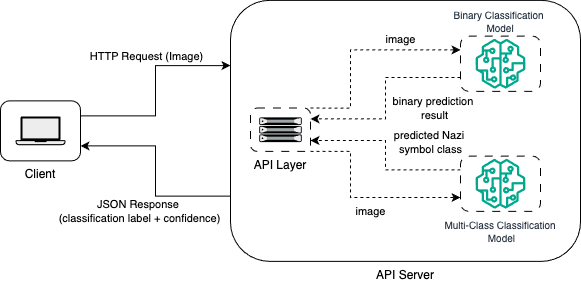
\includegraphics[width=0.7\textwidth]{figures/system_architecture}
    \caption{System architecture of the implemented classification \ac{API} service.}
    \label{fig:system-architecture}
\end{figure}

~\autoref{fig:system-architecture} illustrates the system architecture of the classification \ac{API} service. Users
submit an image file via an HTTP request, which is routed to one of three model pipelines depending on the specified
task: binary classification, multi-class classification, or a two-stage hierarchical classification pipeline.

In the two-stage pipeline, the image is first passed to a binary classifier to determine whether it contains Nazi
symbolism. If no such content is detected, the \ac{API} returns a negative classification. If Nazi-related content
is identified, the image is subsequently forwarded to the multi-class classifier, which predicts the specific type(
s) of Nazi symbol(s), such as swastikas, \ac{SS} bolts, or eagles.

This cascaded design reduces computational overhead for irrelevant inputs and mirrors real-world content moderation
workflows, where fine-grained analysis is only triggered upon initial positive screening.

The backend is implemented using \texttt{FastAPI}. All models are preloaded into memory at service startup, ensuring
low-latency inference. The architecture is stateless and fully containerized, enabling straightforward horizontal
scaling in distributed environments.

\section{Model Integration and Routing Logic}

The \ac{API} exposes distinct endpoints for binary classification, multi-class classification, and the combined
2-layer pipeline. Instead of selecting the model dynamically based on request parameters, each endpoint corresponds
to a specific inference path.

This design simplifies both the server-side routing and the client interface, enabling users to directly interact
with the appropriate endpoint. Each endpoint internally handles preprocessing, model inference, and result formatting.

At service startup, all models are preloaded into memory. \ac{DL} models implemented with PyTorch are
serialized using \texttt{TorchScript}~\footnote{\url{https://pytorch.org/docs/stable/jit.html}} or the standard
PyTorch save format~\footnote{\url{https://pytorch.org/tutorials/beginner/saving_loading_models.html}}.
Classical \ac{ML} models (e.g., logistic regression or \ac{SVC} trained on OpenCLIP embeddings) are serialized using
\texttt{joblib}~\footnote{\url{https://joblib.readthedocs.io/en/latest/}}. This preloading strategy reduces runtime
latency and avoids repeated I/O overhead.

The modular architecture allows easy extension. New models or task-specific pipelines can be integrated by
registering additional routes in the \ac{API} codebase, without disrupting existing functionality.

~\autoref{fig:api-model-routing} summarizes the endpoint-to-model routing logic.

%! Author = zhiweizhang
%! Date = 11.06.25

% Preamble
\begin{figure}[ht]
\centering
\resizebox{\textwidth}{!}{
\begin{tikzpicture}[
    node distance=1.5cm and 2cm,
    every node/.style={font=\small},
    process/.style={rectangle, draw=blue!50, fill=blue!10, thick, minimum width=3.5cm, minimum height=0.9cm},
    endpoint/.style={rectangle, draw=black!80, fill=gray!10, thick, minimum width=4cm, minimum height=0.9cm},
    decision/.style={diamond, aspect=2, draw=red!60, fill=red!10, thick, minimum height=1.2cm},
    response/.style={rectangle, draw=green!50!black, fill=green!10, thick, minimum width=3.5cm, minimum height=0.9cm},
    arrow/.style={->, thick}
]

% API Endpoints
\node[endpoint] (binary) {POST /predict-binary};
\node[endpoint, below=of binary] (multi) {POST /predict-multiclass};
\node[endpoint, below=of multi] (twolayer) {POST /predict};

\node[process, right=of multi] (prep) {Image Preprocessing};

% Two-layer path
\node[decision, right=of prep] (decision) {Contains Nazi Symbol?};
\node[process, right=of decision] (negresponse) {Return: No Symbol};

% Binary path
\node[process, above=2cm of decision] (binarymodel) {Binary Classifier};
\node[response, right=of binarymodel] (binaryresp) {Binary Prediction Response};

% Multi-class path
\node[process, below=2cm of decision] (multimodel) {Multi-Class Classifier};
\node[response, right=of multimodel] (multiresp) {Multi-Class Prediction Response};

\node[response, below right=of multimodel] (finalresp) {Hierarchical Prediction Response};
% Arrows
\draw[red, arrow] (binary.east) -| (prep.150);
\draw[red, arrow] (prep.north) |- (binarymodel.west);
\draw[red, arrow] (binarymodel) -- (binaryresp);

\draw[blue, arrow] (multi) -- (prep);
\draw[blue, arrow] (prep.south) |- (multimodel.west);
\draw[blue, arrow] (multimodel) -- (multiresp);

\draw[arrow] (twolayer.east) -| (prep.-150);
\draw[arrow] (prep) -- (binarymodel);
\draw[arrow] (binarymodel) -- (decision);
\draw[arrow] (decision) -- node[above right] {No} (negresponse);
\draw[arrow] (decision) -- node[below right] {Yes} (multimodel);
\draw[arrow] (multimodel.south) |- (finalresp.west);

\end{tikzpicture}
}
\caption{\ac{API} endpoints mapped to model pipelines, including the 2-layer classification logic.}
\label{fig:api-model-routing}

\end{figure}

\section{Continuous Integration and Deployment}

The service is integrated with a GitHub Actions-based \ac{CI/CD} pipeline, shown in ~\autoref{fig:github-pipeline},
which automates:

\begin{itemize}
    \item Code quality checks and unit testing
    \item Docker image builds and tagging
    \item Generation and deployment of Sphinx-based documentation
    \item Publication of Docker images to Docker Hub
\end{itemize}

Although the \ac{API} is not deployed to a public endpoint, the pipeline ensures that each commit to the main branch
undergoes validation and build procedures, promoting maintainability. Users can reliably pull the latest version
from Docker Hub and execute the service locally or in private cloud environments with minimal setup.

\begin{figure}[ht]
    \centering
    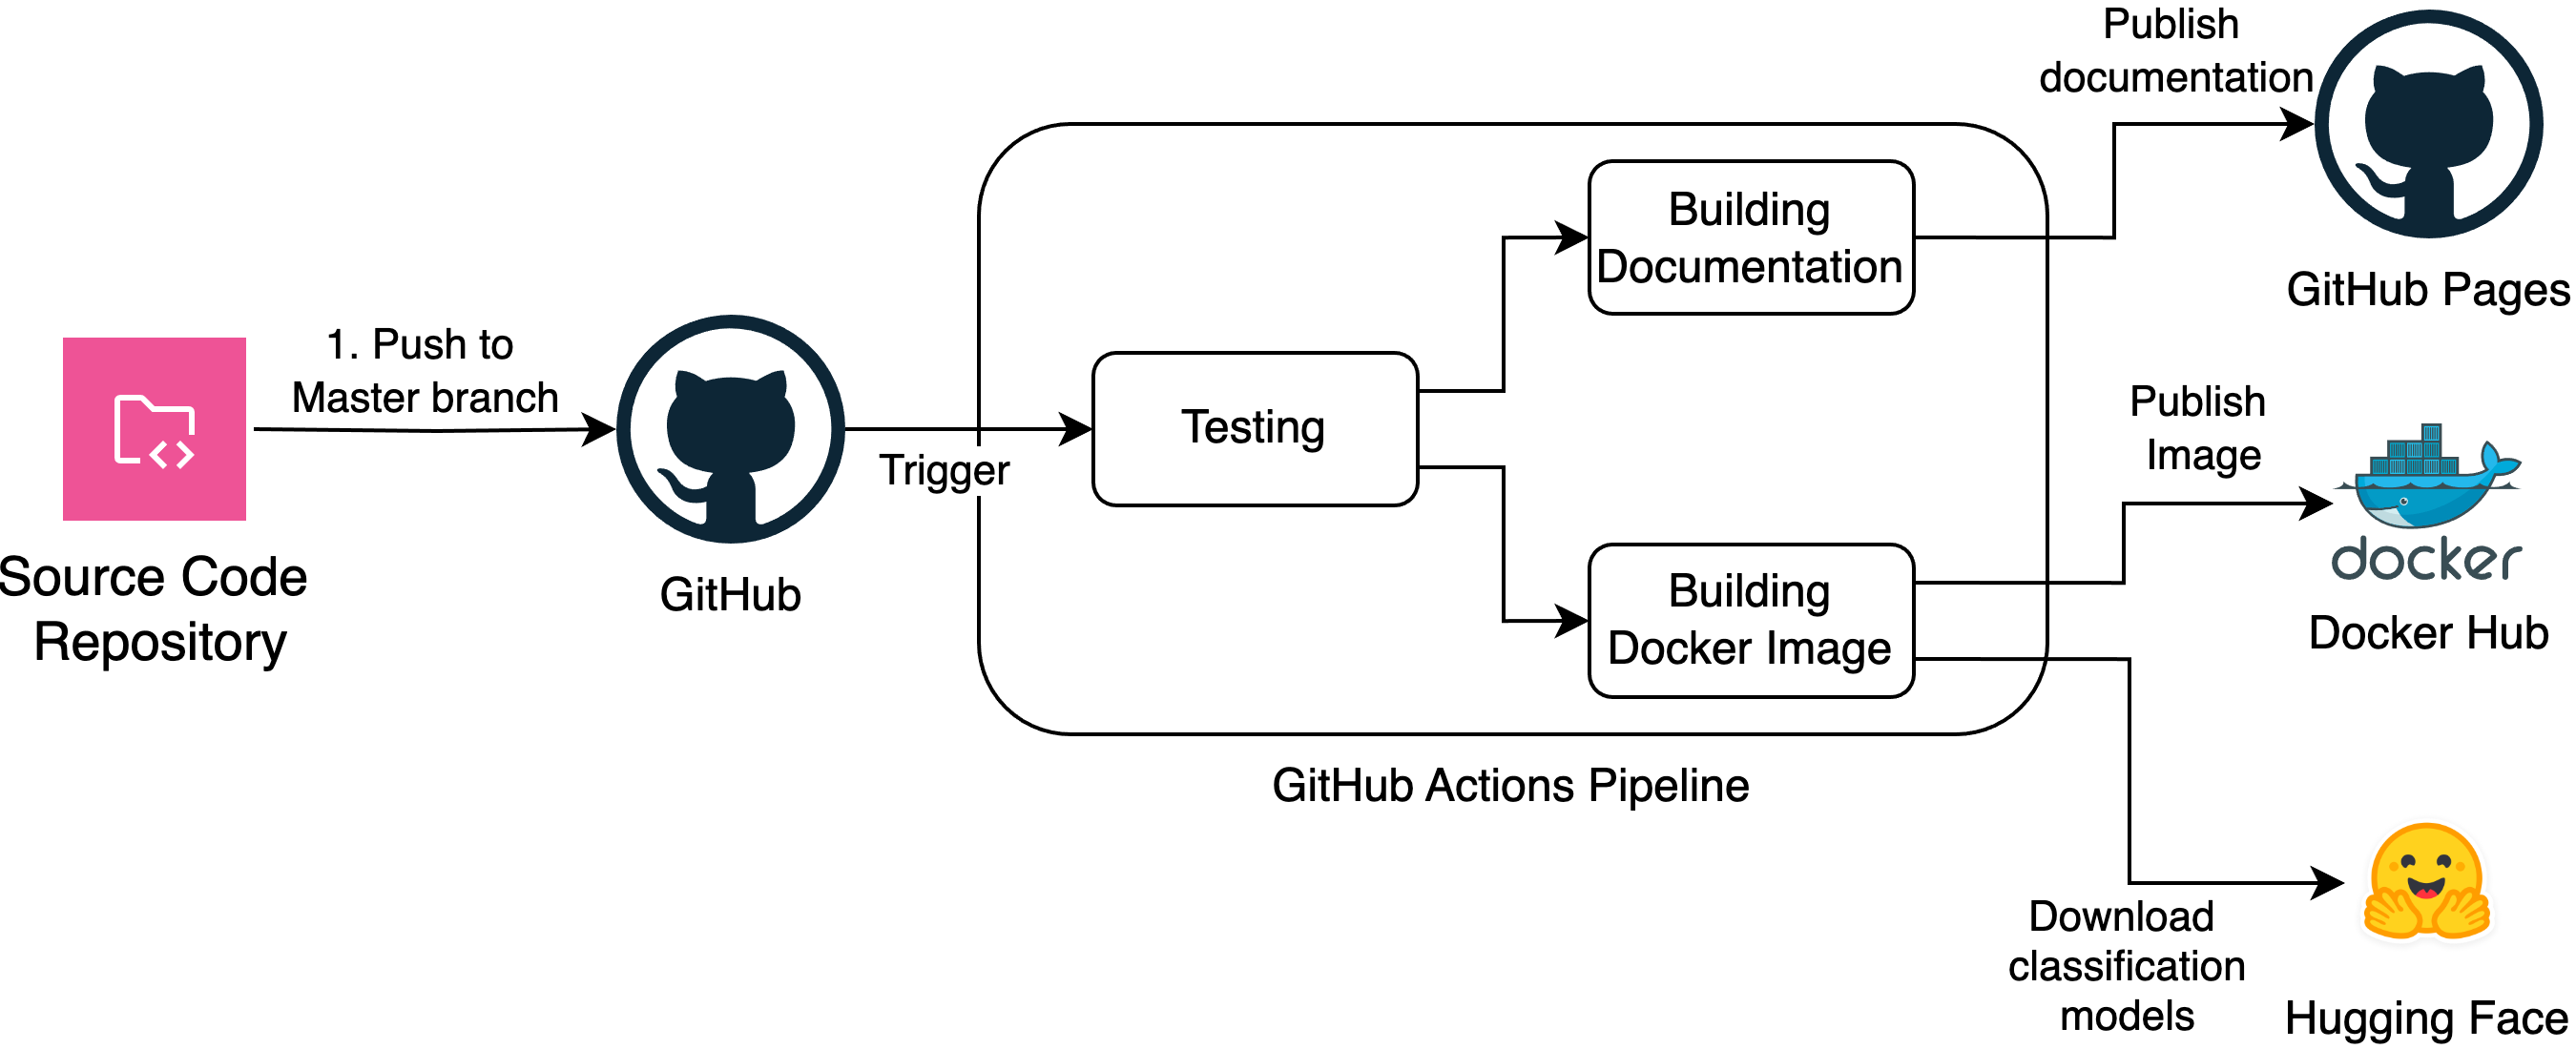
\includegraphics[width=0.7\textwidth]{figures/github_pipeline}
    \caption{GitHub Actions \ac{CI/CD} pipeline for Dockerized \ac{API} service.}
    \label{fig:github-pipeline}
\end{figure}


\section{\ac{API} Endpoints}

\autoref{tab:api-endpoints} summarizes the available endpoints and their functionality.

The 2-layer endpoint encapsulates the binary–multi-class cascade, simplifying client-side logic and supporting
integration into broader moderation or research pipelines.

%! Author = zhiweizhang
%! Date = 10.06.25

% Preamble
\begin{table}[ht]
  \centering
  \resizebox{\textwidth}{!}{
  \begin{tabular}{llp{8cm}}
    \toprule
    \textbf{Method} & \textbf{Endpoint} & \textbf{Description} \\
    \midrule
    \texttt{POST}   & \texttt{/predict} & Runs the 2-layer pipeline: binary classification followed by multi-class prediction if Nazi content is detected. Threshold for symbol inclusion is 0.1. \\
    \texttt{POST}   & \texttt{/predict-binary} & Performs binary classification with associated confidence scores. \\
    \texttt{POST}   & \texttt{/predict-multiclass} & Performs multi-label classification of Nazi symbol types. Returns predictions above confidence threshold 0.1. \\
    \texttt{GET}    & \texttt{/health} & Health check endpoint. \\
    \texttt{GET}    & \texttt{/version} & Returns model and \ac{API} version metadata. \\
    \texttt{GET}    & \texttt{/docs} & Serves OpenAPI documentation via Swagger UI. \\
    \bottomrule
  \end{tabular}
  }
  \caption{Summary of available \ac{API} endpoints.}
  \label{tab:api-endpoints}
\end{table}

All classification endpoints accept images as multipart form data and return structured \ac{JSON} responses. These
responses include predicted classes, confidence scores, and model metadata. The interactive Swagger UI at
\texttt{/docs} facilitates testing and exploration.

\subsection{Example JSON Response}

~\autoref{fig:binary-json-response} shows a sample \ac{JSON} response for the binary classification endpoint.
~\autoref{fig:multi-class-json-response} illustrates a multi-class classification response, while
~\autoref{fig:two-layer-json-response} demonstrates the 2-layer classification response format.

\input{figures/api_responses}

\subsection{Thresholding vs. Top-$k$ in Multi-label Classification}

In the multi-class classification task, images may contain more than one Nazi symbol, constituting a multi-label
problem. Instead of using a top-$k$ strategy, which returns the $k$ most confident classes regardless of absolute
probability, a fixed confidence threshold of 0.1 was used to filter results.

This design offers two key advantages:

\begin{enumerate}
    \item \textbf{Adaptability to Varying Label Counts}: The number of relevant symbols varies across images. A
    threshold-based method allows the model to return only those classes exceeding the confidence threshold, thereby
    adapting to the input's true label count.

    \item \textbf{Reduction of False Positives}: Low-probability predictions are filtered out, reducing the
    likelihood of returning irrelevant or incorrect classifications. This is particularly important in sensitive
    domains such as Nazi symbolism detection, where misclassification could have serious social and legal implications.
\end{enumerate}

This approach provides more nuanced, context-aware predictions and aligns with the goal of responsible content
moderation.

\section{Extensibility and Future Deployment}

The \ac{API} service is architected for extensibility. Future capabilities—such as object detection for symbol
localization, \ac{OCR} for embedded text, or detection of other hate symbols—can be integrated by adding new model
pipelines and routes. The decoupled routing logic and memory preloading facilitate straightforward extensibility.

Although the service is not deployed online, it is fully containerized and ready for local or remote deployment. The
accompanying GitHub repository includes:

\begin{itemize}
    \item A \texttt{Dockerfile} and \texttt{pyproject.toml} for consistent runtime environments
    \item Instructions for local deployment using \texttt{docker run} or \texttt{docker-compose}
    \item Example requests (e.g., via \texttt{curl}) and a Postman collection
    \item GitHub Actions workflows for testing, documentation generation, and Docker publishing
\end{itemize}

This setup supports reproducibility and enables non-technical collaborators (e.g., from social sciences) to run the
service locally without additional configuration.

For future deployment on public platforms, the system could be hosted on AWS, Google Cloud, or Azure. It is
compatible with container orchestration (e.g., Kubernetes) or serverless deployment (e.g., AWS Lambda + \ac{API}
Gateway). Additional features—such as user authentication, request throttling, and secure logging—would be needed
for production-grade deployment.

The modular and portable design ensures that the service can evolve alongside the research project and scale into
production or collaborative use cases as required.



%! Author = zhiweizhang
%! Date = 10.06.25

\chapter{Conclusion and Future Work}\label{chapter:conclusion-and-future-work}

\section{Conclusion}

This thesis presented a comprehensive study on classifying Nazi symbols in images, exploring a wide range of
architectures—including \ac{CNN}s (ResNet and EfficientNet), transformer-based
models (\ac{ViT}), classification-specific versions of \ac{YOLO}, and multimodal approaches leveraging OpenCLIP
embeddings. In addition to end-to-end deep learning pipelines, hybrid approaches that combined OpenCLIP features
with classical \ac{ML} classifiers were also evaluated.

Two classification settings were explored: binary classification (distinguishing Nazi from non-Nazi symbols) and
multi-class classification across 13 Nazi-related symbol categories.

In the binary task, hybrid models—particularly OpenCLIP paired with classical classifiers such as \ac{SVC},
\ac{LR}, KNeighborsClassifier, and SGDClassifier—consistently delivered high performance, achieving F1-scores
above 0.89 and, in some cases, perfect \ac{ROC} \ac{AUC} scores (e.g., \ac{LR} with \ac{AUC} = 1.00). Transformer-based
\ac{ViT} and classification-oriented \ac{YOLO} also demonstrated strong results, balancing accuracy, precision,
and recall. These findings affirm the value of both pre-trained visual-semantic embeddings and end-to-end deep
feature extractors for sensitive symbol classification.

Nonetheless, some hybrid configurations—such as OpenCLIP combined with Decision Tree or Bagging Classifiers—underperformed,
especially in \ac{PR} metrics, signaling limited robustness under class imbalance. Similarly, EfficientNet
achieved high \ac{AUC} (0.993) but lower \ac{AP} (0.780), making it less suitable for applications
requiring fine-grained discrimination.

In the multi-class setting, \ac{YOLO} emerged as the top performer, achieving the highest accuracy, precision, and
F1-score. \ac{ViT} also performed strongly, confirming the effectiveness of global attention mechanisms for nuanced
symbol differentiation. While OpenCLIP performed poorly in zero-shot mode, its performance improved significantly
when combined with supervised classifiers—though still behind end-to-end models. These results highlight the
importance of downstream supervision when applying foundation models to fine-grained classification tasks.

In summary, this work demonstrates that both deep learning and hybrid approaches can be effective for the
classification of Nazi symbols. The choice of model should be guided by task constraints, desired performance
metrics, and deployment requirements. Success ultimately depends on a balance between representational power,
classifier robustness, and sensitivity to class imbalance and symbol diversity—critical considerations for building
practical and ethically responsible systems.


\section{Future Work}

Building on the encouraging results of this study, several key directions for future research emerge:

\paragraph{Dataset Expansion and Balancing:}

Increasing the diversity and quantity of labeled
images—particularly for rare or visually ambiguous Nazi symbols—could significantly improve performance in the
multi-class setting. Incorporating hard negatives (e.g., geometric symbols or cultural motifs that resemble Nazi
iconography) would also enhance binary classifier robustness against false positives.

\paragraph{Fine-Tuning Vision Backbones and Multimodal Retraining:}
While OpenCLIP embeddings paired with
classical classifiers showed strong performance, they were limited in zero-shot generalization. Task-specific
fine-tuning of the OpenCLIP vision encoder—or end-to-end multimodal retraining with labeled Nazi symbol data—may
lead to better feature separability and improved recall across all classes.

\paragraph{Precision-Focused Learning Objectives:}
As shown in the results, high \ac{AUC} did not always
translate into high real-world precision. Future work could experiment with cost-sensitive loss functions,
confidence calibration, or threshold tuning to explicitly optimize for precision-recall trade-offs—especially
important in applications with legal or reputational risks.

\paragraph{Explainability and Human Oversight:}
Integration of explainable AI (XAI) tools such as
\ac{Grad-CAM}~\parencite{Selvaraju_2019} or \ac{SHAP}~\parencite{SHAP2025} would improve transparency and
accountability. Providing visual or textual explanations for predictions could support expert review and
increase user trust—especially in archival or forensic applications.

\paragraph{Contextual and Multimodal Classification:}
Some misclassifications were driven by lack of context.
Incorporating auxiliary metadata (e.g., captions, filenames, web text) and exploring multimodal fusion models
could improve classification of ambiguous or reused symbols, and help distinguish educational versus
propagandistic usage.

\paragraph{Real-Time Deployment and System Scalability:}
Future engineering work should extend the current
containerized \ac{API} toward production-ready deployment. Key goals include low-latency inference,
cross-platform scalability, and compliance with privacy regulations (e.g., GDPR), making the system usable in
content moderation or institutional archiving workflows.

\paragraph{Human-in-the-Loop Feedback and Adaptation:}
Building mechanisms for expert feedback and iterative
improvement would support continuous learning. This is especially valuable in evolving symbol ecosystems where
new variants or context-specific uses emerge over time.


In summary, future efforts should aim to enhance the system’s precision, transparency, and adaptability to sensitive real-world environments. By combining improved data practices, targeted fine-tuning, explainability, and user input, the classifier can evolve into a more trustworthy and context-aware tool for ethical Nazi symbol recognition and moderation.


% TODO: add more chapters here

\appendix{}

\microtypesetup{protrusion=false}

\addchap{Abbreviations}
\begin{acronym}
	\itemsep-.25\baselineskip
	\acro{TUM}[TUM]{Technical University of Munich}
	% TODO: add acronyms
	\acro{ViT}[ViT]{Vision Transformer}
	\acro{LR}[LR]{Logistic Regression}
	\acro{CNN}[CNN]{Convolutional Neural Network}
	\acro{ML}[ML]{Machine Learning}
	\acro{CI/CD}[CI/CD]{Continuous Integration/Continuous Delivery}
	\acro{DL}[DL]{Deep Learning}
	\acro{VGGNet}[VGGNet]{Visual Geometry Group Network}
	\acro{ZSL}[ZSL]{Zero-Shot Learning}
	\acro{CLIP}[CLIP]{Contrastive Language-Image Pre-training}
	\acro{RN}[RN]{Relation Network}
	\acro{AI}[AI]{Artifical Intelligence}
	\acro{BiLSTM}[BiLSTM]{Bidirectional Long Short-Term Memory}
	\acro{ADL}[ADL]{Anti-Defamation League}
	\acro{BUF}[BUF]{British Union of Fascists}
	\acro{SA}[SA]{Sturmabteilung}
	\acro{SS}[SS]{Schutzstaffel}
	\acro{NOP}[NOP]{National Rebirth of Poland}
	\acro{YOLO}[YOLO]{You Only Look Once}
	\acro{ResNet}[ResNet]{Residual Network}
	\acro{SotA}[SotA]{state of the art}
	\acro{NLP}[NLP]{Natual Language Processing}
	\acro{KNN}[KNN]{K-Nearest Neighbors}
	\acro{SVC}[SVC]{Support Vector Classifier}
	\acro{SGD}[SGD]{Stochastic Gradient Descent}
	\acro{BCE}[BCE]{Binary cross-entropy}
	\acro{CCE}[CCE]{categorical cross-entropy}
	\acro{NAdam}[NAdam]{Nesterov momentum variant of Adam}
	\acro{AUC-ROC}[AUC-ROC]{Area Under the ROC Curve}
	\acro{TPR}[TPR]{True Positive Rate}
	\acro{FPR}[FPR]{False Positive Rate}
	\acro{ROC}[ROC]{Receiver Operating Characteristic}
	\acro{AP}[AP]{Average Precision}
	\acro{PR}[PR]{Precision-Recall}
	\acro{AUC}[AUC]{Area under the curve}
	\acro{API}[API]{Application Programming Interface}
	\acro{REST}[REST]{Representational State Transfer}
	\acro{JSON}[JSON]{JavaScript Object Notation}
	\acro{OCR}[OCR]{Optical character recognition}
	\acro{XAI}[XAI]{explainable AI}
	\acro{SHAP}[SHAP]{SHapley Additive exPlanations}
	\acro{Grad-CAM}[Grad-CAM]{Gradient-weighted Class Activation Mapping}
	\acro{GDPR}[GDPR]{General Data Protection Regulation}
	\acro{PII}[PII]{personally identifiable information}
	\acro{DFG}[DFG]{Deutsche Forschungsgemeinschaft}
	\acro{IEEE}[IEEE]{Institute of Electrical and Electronics Engineers}
	\acro{UNESCO}[UNESCO]{United Nations Educational, Scientific and Cultural Organization}
\end{acronym}

\listoffigures{}
\listoftables{}
\microtypesetup{protrusion=true}
\printbibliography{}

\end{document}
